%%% Hlavní soubor. Zde se definují základní parametry a odkazuje se na ostatní části. %%%

% Meta-data o práci (je nutno upravit)
\input metadata.tex

% Vygenerujeme metadata ve formátu XMP pro použití balíčkem pdfx
\input xmp.tex

%% Verze pro jednostranný tisk:
% Okraje: levý 40mm, pravý 25mm, horní a dolní 25mm
% (ale pozor, LaTeX si sám přidává 1in)
\documentclass[12pt,a4paper]{report}
\setlength\textwidth{145mm}
\setlength\textheight{247mm}
\setlength\oddsidemargin{15mm}
\setlength\evensidemargin{15mm}
\setlength\topmargin{0mm}
\setlength\headsep{0mm}
\setlength\headheight{0mm}
% \openright zařídí, aby následující text začínal na pravé straně knihy
\let\openright=\clearpage

%% Pokud tiskneme oboustranně:
% \documentclass[12pt,a4paper,twoside,openright]{report}
% \setlength\textwidth{145mm}
% \setlength\textheight{247mm}
% \setlength\oddsidemargin{14.2mm}
% \setlength\evensidemargin{0mm}
% \setlength\topmargin{0mm}
% \setlength\headsep{0mm}
% \setlength\headheight{0mm}
% \let\openright=\cleardoublepage

%% Pokud práci odevzdáváme pouze elektronicky, vypadají lépe symetrické okraje
% \documentclass[12pt,a4paper]{report}
% \setlength\textwidth{145mm}
% \setlength\textheight{247mm}
% \setlength\oddsidemargin{10mm}
% \setlength\evensidemargin{10mm}
% \setlength\topmargin{0mm}
% \setlength\headsep{0mm}
% \setlength\headheight{0mm}
% \let\openright=\clearpage

%% Vytváříme PDF/A-2u
\usepackage[a-2u]{pdfx}

%% Přepneme na českou sazbu a fonty Latin Modern
\usepackage[czech]{babel}
\usepackage{lmodern}

% Pokud nepouživáme LuaTeX, je potřeba ještě nastavit kódování znaků
\usepackage{iftex}
\ifpdftex
\usepackage[utf8]{inputenc}
\usepackage[T1]{fontenc}
\usepackage{textcomp}
\fi

%%% Další užitečné balíčky (jsou součástí běžných distribucí LaTeXu)
\usepackage{amsmath}        % rozšíření pro sazbu matematiky
\usepackage{amsfonts}       % matematické fonty
\usepackage{amsthm}         % sazba vět, definic apod.
\usepackage{bm}             % tučné symboly (příkaz \bm)
\usepackage{booktabs}       % lepší vodorovné linky v tabulkách
\usepackage{caption}        % umožní definovat vlastní popisky plovoucích objektů
\usepackage{csquotes}       % uvozovky závislé na jazyku
\usepackage{dcolumn}        % vylepšené zarovnání sloupců tabulek
\usepackage{floatrow}       % umožní definovat vlastní typy plovoucích objektů
\usepackage{graphicx}       % vkládání obrázků
\usepackage{icomma}         % inteligetní čárka v matematickém módu
\usepackage{indentfirst}    % zavede odsazení 1. odstavce kapitoly
\usepackage[nopatch=item]{microtype}  % mikrotypografická rozšíření
\usepackage{paralist}       % lepší enumerate a itemize
\usepackage[nottoc]{tocbibind} % zajistí přidání seznamu literatury,
                            % obrázků a tabulek do obsahu
\usepackage{xcolor}         % barevná sazba

% Balíček hyperref, kterým jdou vyrábět klikací odkazy v PDF,
% ale hlavně ho používáme k uložení metadat do PDF (včetně obsahu).
% Většinu nastavítek přednastaví balíček pdfx.
\hypersetup{unicode}
\hypersetup{breaklinks=true}

% Balíčky pro sazbu informatických prací
\usepackage{algpseudocode}  % součást balíčku algorithmicx
\usepackage[Algoritmus]{algorithm}
\usepackage{fancyvrb}       % vylepšené prostředí verbatim
\usepackage{listings}       % zvýrazňování syntaxe zdrojových textů

% Cleveref může zjednodušit odkazování, ale jeho užitečnost pro češtinu
% je minimalní, protože nezvládá skloňování.
% \usepackage{cleveref}

% Formátování bibliografie (odkazů na literaturu)
% Detailní nastavení můžete upravit v souboru macros.tex.
%
% POZOR: Zvyklosti různých oborů a kateder se liší. Konzultujte se svým
% vedoucím, jaký formát citací je pro vaši práci vhodný!
%
% Základní formát podle normy ISO 690 s číslovanými odkazy
\usepackage[natbib,style=iso-numeric,sorting=none]{biblatex}
% ISO 690 s alfanumerickými odkazy (zkratky jmen autorů)
%\usepackage[natbib,style=iso-alphabetic]{biblatex}
% ISO 690 s citacemi tvaru Autor (rok)
%\usepackage[natbib,style=iso-authoryear]{biblatex}
%
% V některých oborech je běžnější obyčejný formát s číslovanými odkazy
% (sorting=none říká, že se bibliografie má řadit podle pořadí citací):
%\usepackage[natbib,style=numeric,sorting=none]{biblatex}
% Číslované odkazy, navíc se [1,2,3,4,5] komprimuje na [1-5]
%\usepackage[natbib,style=numeric-comp,sorting=none]{biblatex}
% Obyčejný formát s alfanumerickými odkazy:
%\usepackage[natbib,style=alphabetic]{biblatex}

% Z tohoto souboru se načítají položky bibliografie
\addbibresource{literatura.bib}

% Definice různých užitečných maker (viz popis uvnitř souboru)
\input macros.tex

%%% Titulní strana a různé povinné informační strany
\begin{document}
%%% Titulní strana práce a další povinné informační strany

%%% Nápisy na přední straně desek
%%% Pokud je práce ve slovenštině, desky mají být česky.

% Desky obvykle nesázíme, ale pokud je chcete přidat, změnte \iffalse na \iftrue
\iffalse

\pagestyle{empty}
\hypersetup{pageanchor=false}
\begin{center}

\large
Univerzita Karlova

\medskip

Matematicko-fyzikální fakulta

\vfill

{\huge\bf\ThesisTypeTitle}

\vfill

{\huge\bf\ThesisTitle\par}

\vfill
\vfill

\hbox to \hsize{\YearSubmitted\hfil \ThesisAuthor}

\end{center}

\newpage\openright
\setcounter{page}{1}

\fi

%%% Titulní strana práce
%%% Pokud je práce ve slovenštině, tato strana zůstává česky.

\pagestyle{empty}
\hypersetup{pageanchor=false}

\begin{center}

\centerline{\mbox{
\includegraphics[width=166mm]{img/logo-cs.pdf}}}

\vspace{-8mm}
\vfill

{\bf\Large\ThesisTypeTitle}

\vfill

{\LARGE\ThesisAuthor}

\vspace{15mm}

{\LARGE\bfseries\ThesisTitle\par}

\vfill

\Department

\vfill

{
\centerline{\vbox{\halign{\hbox to 0.45\hsize{\hfil #}&\hskip 0.5em\parbox[t]{0.45\hsize}{\raggedright #}\cr
Vedoucí \ThesisTypeGenitive{} práce:&\Supervisor \cr
\ifx\ThesisType\TypeRig\else
\noalign{\vspace{2mm}}
Studijní program:&\StudyProgramme \cr
\fi
}}}}

\vfill

Praha \YearSubmitted

\end{center}

\newpage

%%% Strana s čestným prohlášením k práci
%%% Pokud je práce ve slovenštině, tato strana zůstává česky.

\openright
\hypersetup{pageanchor=true}
\vglue 0pt plus 1fill

\noindent
Prohlašuji, že jsem tuto \ThesisTypeAccusative{} práci vypracoval samostatně a výhradně
s~použitím citovaných pramenů, literatury a dalších odborných zdrojů.
Beru na~vědomí, že se na moji práci vztahují práva a povinnosti vyplývající
ze zákona č. 121/2000 Sb., autorského zákona v~platném znění, zejména skutečnost,
že Univerzita Karlova má právo na~uzavření licenční smlouvy o~užití této
práce jako školního díla podle §60 odst. 1 autorského zákona.

\vspace{10mm}

\hbox{\hbox to 0.5\hsize{%
V \hbox to 6em{\dotfill} dne \hbox to 6em{\dotfill}
\hss}\hbox to 0.5\hsize{\dotfill\quad}}
\smallskip
\hbox{\hbox to 0.5\hsize{}\hbox to 0.5\hsize{\hfil Podpis autora\hfil}}

\vspace{20mm}
\newpage

%%% Poděkování

\openright

\noindent
\Dedication

\newpage

%%% Povinná informační strana práce

\openright
{\InfoPageFont

\vtop to 0.5\vsize{
\setlength\parindent{0mm}
\setlength\parskip{5mm}

Název práce:
\ThesisTitle

Autor:
\ThesisAuthor

\DeptType:
\Department

Vedoucí \ThesisTypeGenitive{} práce:
\Supervisor, \SupervisorsDepartment

Abstrakt:
\Abstract

Klíčová slova:
{\def\sep{\unskip, }\ThesisKeywords}

\vfil
}

\vtop to 0.49\vsize{
\setlength\parindent{0mm}
\setlength\parskip{5mm}

Title:
\ThesisTitleEN

Author:
\ThesisAuthor

\DeptTypeEN:
\DepartmentEN

Supervisor:
\Supervisor, \SupervisorsDepartmentEN

Abstract:
\AbstractEN

Keywords:
{\def\sep{\unskip, }\ThesisKeywordsEN}

\vfil
}

}

\newpage

%%% Další stránky budeme číslovat
\pagestyle{plain}


%%% Strana s automaticky generovaným obsahem práce

\tableofcontents

%%% Jednotlivé kapitoly práce jsou pro přehlednost uloženy v samostatných souborech
\chapter*{Úvod}
\addcontentsline{toc}{chapter}{Úvod}

Veľmi často v živote narážame na~situácie, kedy sa potrebujeme dostať z~bodu A do~bodu B čo najrýchlejším spôsobom. V~mnohých prípadoch máme k~dispozícii sieť cestných komunikácii či~chodníkov, na~základe ktorých sa môžeme rozhodovať, ktorá trasa je pre~nás vyhovujúca. Pre~takéto prípady nám veľmi dobre poslúžia už existujúce navigačné systémy, ktoré~majú podrobne zmapovanú cestné siete a~vedia nám na~základe parametrov týchto ciest určiť najrýchlejšiu alebo~najúspornejšiu trasu.

Avšak môžu nastať aj~situácie, kedy je cestná sieť priveľmi riedka, až takmer neprítomná. Väčšinou takéto situácie nastávajú vo~voľnej prírode a~oblastiach ďaleko od civilizácie. V~takých prípadoch nám konvenčné navigácie veľmi dobre neposlúžia. Ak máme k~dispozícii kvalitnú mapu, môžeme sa pokúsiť v nej nájsť vyhovujúcu trasu vlastnými silami, ale~často existuje príliš mnoho možností, ktorými sa môžeme vydať. Preto by sa niekedy hodilo mať nástroj, ktorý~na~základe zadaných parametrov nájde na~predloženej mape najrýchlejšiu trasu, po~ktorej sa človek môže vydať k~vytýčenému cieľu.

Príklady využitia takéhoto software-u by sme mohli nájsť v špecifických profesiách ako sú napríklad lesníctvo, záchranné služby či~ozbrojené sily. V~týchto profesiách je niekedy potrebné dostať sa na~odľahlé miesto, aby~bolo možné vykonať ich zámery.

Software by však našiel uplatnenie taktiež v rekreačných aktivitách, ako sú turizmus a~šport, ktoré~sa často odohrávajú vo~voľnej prírode. Z~rôznych dôvodov sa potom môže zísť schopnosť nájdenia najrýchlejšej trasy späť do~najbližšej obývanej oblasti, či~už za~alebo~bez~pomoci ciest. 

Rád by som vyzdvihol špecificky jedno športové odvetvie, ktoré~veľmi úzko súvisí s~hľadaním ciest v otvorenom teréne a~to \textit{orientačný beh}. \uv{Orientačný beh (skratka OB) je športové odvetvie vytrvalostného charakteru, pri~ktorom je úlohou prejsť alebo~prebehnúť podľa mapy a~buzoly trať vyznačenú na~mape za~čo najkratší čas. V~teréne nie je trať vyznačená, sú tam umiestnené iba kontrolné stanovišťa (Kontroly)}\cite{CoJeOrientak}. Tento šport bol hlavnou motiváciou pre~vytvorenie aplikácie, v ktorej by si užívateľ mohol nechať vykresliť na~mape najrýchlejší postup pre~ním zadanú trať. 

\bigskip

V~tejto práci sú popísané myšlienky použité pri~vytváraní spomínanej aplikácie, jej architektúry a~implementácie.

V~prvej kapitole je možné nájsť abstrakciu nad samotnou problematikou hľadania najrýchlejšej trasy v otvorenom teréne podľa konkrétnej mapy. Táto abstrakcia je poňatá z~pohľadu orientačného behu. Ďalej je v nej možné nájsť informácie o~využitých prostriedkoch pri~implementácii aplikácie. Týmito prostriedkami sú napríklad využívaný jazyk a~knižnice, ale~aj~použitý návrhový vzor architektúry aplikácie. 

V~následujúcej kapitole je predostretý bližší pohľad na~spomínanú architektúru aplikácie, jej \uv{horizontálne} a~\uv{vertikálne} členenie na~vrstvy. Funkcie a~správanie jednotlivých vrstiev sú v tejto kapitole dopodrobna vysvetlené.

V~tretej kapitole sa pozrieme na~aktuálne existujúce vertikálne vrstvy aplikácie. Ich funkciu a~architektúru popíšeme po~jednotlivých častiach. Popíšeme špecifické vlastnosti a~spôsoby použitia týchto častí. 

Vo štvrtej a~zároveň poslednej kapitole bude možný k~nahliadnutiu popis horizontálnej vrstvy zvanej \textit{Model}. Táto vrstva sa delí na~mnoho oblastí, z~ktorých každá spravuje určitý typ dát a~mechanizmov využívaných vo~zvyšných vrstvách aplikácie. Štruktúra implementácií jednotlivých oblastí bude v tejto kapitole detailne rozobraná.

Nakoniec v Prílohe~\ref{uzivatelska_dokumentacia} je možné nahliadnuť užívateľskú dokumentáciu ku aplikácii, ktorá~popisuje základy jej používania.

Súčasťou bakalárskej práce sú taktiež elektronické prílohy, ktoré~boli spoločne s~textom pridané do~\textit{Studijního informačního systému} (SIS) Karlovej univerzity. Tieto prílohy zahŕňajú:
\begin{itemize}
    \item Zdrojový kód vytvorenej aplikácie.
    \item Vygenerovanú programátorskú dokumentáciu na~základe dokumentačných komentárov v~zdrojovom kóde.
    \item Ukážkové súbory s~mapami a~užívateľským modelom.  
\end{itemize}



\chapter{Obecné informácie o aplikácii}

\section{Aspekty hľadania najrýchlejšej trasy (v OB)}\label{Aspekty_hladania}

Mapy pre orientačný beh sú veľmi detailné a bežec má preto mnoho informácií na to, aby si mohol zvoliť ideálnu trasu. Za predpokladu, že bežec nerobí chyby a beží presne podľa svojho zámeru, sú pre výber najrýchlejšieho postupu dôležité dva druhy objektov: líniové (cesty, potoky, prieseky, ...) a plošné (lúky, kroviská, vodné objekty, močiare, ...). Tie určujú typ terénu nachádzajúci sa v danej časti mapy a tým pádom aj veľkosť odporu, ktorý je kladený rýchlosti behu pretekára. Táto veličina sa dá použiť ako hlavný parameter, ktorý bude určovať preferencie výberu postupu.

Proces hľadania cesty sa skladá z dvoch hlavných častí: 
\begin{itemize}
    \item \textbf{vytvorenie mapovej reprezentácie} - Na začiatku je potrené na základe mapového súboru vygenerovať mapovú reprezentáciu, na ktorej bude možné cestu vyhľadávať. Mapovou reprezentáciou by mal byť objekt, ktorý dobre vystihne topografiu mapy a umožní hľadanie najideálnejšej trasy. V našej aplikácii budú týmito objektmi \textit{ohodnotené grafy}.  
    \item \textbf{aplikácia vyhľadávacieho algoritmu} - mapová reprezentácia je predaná algoritmu a on za použitia jej interface-u v nej vyhľadá najkratšiu cestu. V našom prípade najkratšia cesta znamená tá najrýchlejšia.
\end{itemize}

V následujúcich podsekciách spomeniem koncepty, ktoré budú v procese hľadania najrýchlejších ciest vystupovať. Medzi jednotlivými konceptmi sú tvorené rôzne závislosti. Grafické znázornenie týchto závislostí je možné nahliadnuť na konci sekcie v obrázku \ref{obr01:konceptove_zavislosti}.   

\subsection{Mapy}\label{mapy}

Na začiatok je potrebné spomenúť koncept mapy. V procese hľadania ciest bude na viacerých miestach potrebné agregovať dáta z užívateľom vybraného mapového súboru. Aby sme nemuseli neustále čítať priamo zo súboru, budeme si udržovať jeho obsah v pamäti prívetivejším spôsobom. 

Touto formou bude práve \textit{mapa}. Mapa si bude udržovať všetky objekty definované v mapovom súbore a keď bude potrebné agregovať z daného súboru nejakú informáciu (mapovú reprezentáciu, mapovú grafiku, ...), použije sa namiesto súboru odpovedajúci mapový objekt.

Je vhodné zmieniť, že koncept mapy je odlišný od konceptu \textit{mapovej reprezentácie}. Mapa, na rozdiel od jej reprezentácie, neobsahuje žiadne zložité prepojenia medzi objektami ktoré v sebe drží. Jej vytvorenie by malo byť rýchle, s lineárnou časovou zložitosťou v závislosti na veľkosti mapového súboru.

\subsection{Mapové reprezentácie}\label{mapove_reprezentacie}

Mapové reprezentácie sú jednou z dôležitých zložiek procesu hľadania ciest. Sú to jednotky, na ktorých sa vyhľadávanie uskutočňuje. Mapové objekty sú oproti \textit{mapám} zložitejšie objekty, ktoré už v sebe zahrňujú plno závislostí a prepojení. Ich generovanie môže zabrať oveľa viac času ako generovanie mapových objektov. 

Ako už bolo spomenuté vyššie, v aplikácii budú mapovými reprezentáciami \textit{ohodnotené grafy} (naďalej iba grafy). Napriek tomu, že mapová reprezentácia a graf budú v aplikácii reprezentovať rovnaký objekt, ich významy sú odlišné:

\begin{itemize}
    \item \textbf{Mapová reprezentácia} hovorí o tom, ako daný objekt pracuje interne. Popisuje jeho vlastnosti, mechanizmy a spôsoby akými generuje výsledný \textit{graf}, v ktorom sa následne hľadá cesta. Objekt, ktorý je agregovaný z mapy, je v prvom rade mapovou reprezentáciou a až v druhom rade grafom.
    
    Príkladom myšlienky, ktorú môže mapová reprezentácia vyjadrovať je \uv{samo-zahusťujúci} sa graf. Takáto mapová reprezentácia počas behu algoritmu zahusťuje predom pripravený graf o ďalšie vrcholy na miestach, v ktorých sa prehľadávanie aktuálne uskutočňuje. Redukuje sa tým veľkosť vygenerovaného grafu.   
    \item\textbf{Graf} na druhej strane hovorí o vlastnostiach objektu, ktoré sú viditeľné navonok. Bude informovať o \uv{grafových} službách objektu, ktoré dokáže poskytnúť. Tieto služby môžu byť obmedzené práve vnútornou štruktúrou ktorá je definovaná \textit{mapovou reprezentáciou}. Graf sa berie ako druhotný produkt spracovania mapy.   

    Príkladom vlastnosti, ktorú môže graf prezentovať vonkajšiemu svetu, je možnosť poskytnutia kompletne vygenerovaného grafu, pri ktorom sa vonkajší užívateľ nemusí obávať, že by sa počas práce s ním graf nejakým spôsobom modifikoval. Túto vlastnosť napríklad nevie zaručiť graf ktorý zodpovedá vyššie zmienenej mapovej reprezentácii, ktorá stav grafu počas práce neustále modifikuje, zahusťuje ho.
\end{itemize}

Pojmy \textit{mapová reprezentácia} a \textit{graf} budú naďalej v práci brané ako zameniteľné a ich použitie bude závisieť od okolitého kontextu a ich špecifického významu.

\subsection{Užívateľské modely}\label{uzivatelske_modely}

Je potrebné si uvedomiť, že rôzni bežci majú rôzne schopnosti a preto aj ich preferencie na výber trasy nemusia byť rovnaké. Niekto sa dokáže rýchlejšie predierať cez husté pasáže, inému ide rýchlejšie beh cez močiar a ďalšiemu vyhovujú dlhšie postupy po cestách. 

Preto by bolo vhodné, aby užívateľ aplikácie mal možnosť aplikovať svoje preferencie do procesu vyhľadávania. K tomuto účelu boli vytvorené tzv. \uv{užívateľské modely}. Užívateľ si pomocou nich môže vytvoriť vlastný \uv{profil}, na základe ktorého bude vyhľadávanie cesty prispôsobené.

Užívateľské modely vďaka svojej informovanosti nadobúdajú zodpovednosť za výpočty hodnôt, ktoré sú závislé na preferenciách užívateľa. Stávajú sa teda dôležitou zložkou procesu vyhľadávania ciest. Vyhľadávacie algoritmy stávajú závislé na nimi vykonávaných výpočtoch.

\subsection{Výškové dáta}\label{vyskove_data}

Jedným z dôležitých a neopomenuteľných faktorov voľby najrýchlejšieho postupu je prevýšenie, ktoré je potrebné pri jeho prevedení zdolať. Mnoho typov máp popisuje reliéf krajiny pomocou takzvaných \textit{vrstevníc}. Vrstevnica je krivka na mape, ktorá spája body rovnakej nadmorskej výšky. Pre človeka je vrstevnicová abstrakcia výšky terénu veľmi ľahko pochopiteľná a spracovateľná.

Pre strojové spracovanie mapy však vrstevnice predstavujú veľmi neprirodzený spôsob reprezentácie nadmorskej výšky. Vypracovanie reliéfneho obrazu za pomoci vrstevníc samotných je veľmi ťažká úloha. V niektorých prípadoch (mapy pre OB napríklad) dokonca jednotlivé vrstevnice nie sú v mapovom súbore reprezentované jedným objektom, nakoľko kvôli dobrej čitateľnosti máp sú na viacerých miestach prerušované.
%TODO: mozno najst nejaku tu pracu co sa tym zaoberala, zistit od risa, odkazat na nu

Z vyššie uvedených dôvodov je v aplikácii zahrnutý systém, ktorý sprostredkováva užívateľom možnosť stiahnutia a spravovania digitálnych výškových dát, ktoré následne môžu byť použité ako pomocný zdroj v procese tvorby mapových reprezentácií. Pre konštrukciu mapových reprezentácií pre niektoré mapové formáty bude nutná prítomnosť zodpovedajúcich výškových dát a pri ich absencii jednoducho nebude možné mapové reprezentácie vytvoriť.

Výškové dáta môžu byť sťahované z viacerých zdrojov. Každý zdroj môže definovať viacero dátových distribúcií, ktoré dokáže ponúknuť. Tieto distribúcie sa väčšinou líšia kvalitou a dostupnosťou sprostredkovaných dát (v niektorých prípadoch je ku možnosti stiahnutia výškových dát potrebná užívateľova autorizácia).

\subsection{Atribútové template-y}\label{templatey}

Ďalšia vec, nad ktorou je potrebné sa zamyslieť je, akým spôsobom sa bude v grafoch mapových reprezentácií uchovávať informácia o mapových vlastnostiach a atribútoch, ktoré konkrétne vrcholy a hrany grafu reprezentujú. Zároveň je potrebné aby dotyčné vlastnosti dokázal príslušný užívateľský model spracovať a dopočítať z nich hodnoty, potrebné pre beh vyhľadávacích algoritmov. Používané atribúty, ktoré agregujeme z máp do mapových reprezentácií preto musia byť jednotné v celom procese hľadania cesty, od vytvárania mapovej reprezentácie, po spustenie vyhľadávacieho algoritmu.

V aplikácii nám definíciu a jednotnosť atribútov budú zabezpečovať tzv. \textit{template}-y. Každý template bude definovať jedinečnú sadu vrcholových a hranových atribútov. Príkladom pre takúto kolekciu pre potreby OB môže byť napríklad:
\begin{itemize}
    \item vrcholové atribúty - pozícia, výška, indikátory reprezentovaných terénnych objektov (či sa daný vrchol nachádza na ceste, v húštine, na lúke, v dobre priebežnom lese,...)
    \item hranové atribúty - či daná hrana reprezentuje úsek nejakej cesty, hranu nejakého objektu(lúky, húštiny, močiaru,...), sklon terénu
\end{itemize}

Na template-och ako takých bude teda závisieť: 
\begin{itemize}
    \item \textbf{výber užívateľských modelov} - model musí vedieť spracovať atribúty definované daným template-om a vrátiť od neho požadované výsledky.
    \item \textbf{formát vybraného mapového súboru} - musí existovať konvertor mapy špecifického formátu na odpovedajúcu mapovú reprezentáciu, v ktorej vrcholoch a hranách sú obsiahnuté atribúty definované daným template-om. Túto závislosť môžeme brať aj opačným smerom - pre vybraný mapový formát môžeme zvoliť len použiteľný template.
\end{itemize}

\subsection{Vyhľadávacie algoritmy}\label{vyhladavacie_algoritmy}

Nakoniec nemôžeme opomenúť koncept samotných vyhľadávacích algoritmov, poslednú neodmysliteľnú súčasť procesu hľadania ciest. Vyhľadávací algoritmus, podobne ako \textit{mapová reprezentácia}, reprezentuje koncept vnútorného mechanizmu ktorým je najkratšia cesta v grafe hľadaná. Príkladom takéhoto algoritmu môže byť napríklad algoritmus \textit{A*}. 

Vstupom do každého algoritmu sú:
\begin{itemize}
    \item \textbf{graf}, na ktorom je hľadanie najkratšej cesty vykonané a 
    \item \textbf{užívateľský model}, ktorý algoritmus nutne potrebuje ku výpočtom váh grafových hrán a iných hodnôt potrebných k jeho správnemu chodu.  
\end{itemize}

Každý algoritmus následne ponúka množinu jeho implementácií. Každá implementácia definuje množinu vlastností, ktoré vložený graf a užívateľský model musia spĺňať. Napríklad implementácie A* algoritmu budú požadovať, aby užívateľský model bol schopný, popri výpočte váh pre grafové hrany, dodať ešte aj výpočet heuristiky využívanej v týmto algoritmom.

Stav používaného grafu sa môže počas behu algoritmu meniť. Teda je potrebné ho vždy na konci vyhľadávania opäť vrátiť do pôvodného stavu a zaručiť, že graf je v jednu chvíľu súčasťou len jedného vyhľadávacieho procesu.

Vyhľadávanie samotné je sprostredkované dvomi spôsobmi. Buď sa požiada algoritmus priamo o nájdenie cesty na danej trati alebo sa využije takzvaný \textit{executor} algoritmu. 

Executor nám sprostredkuje vybraný algoritmus, ktorý bude pracovať s dodanou mapovou reprezentáciou a užívateľským modelom. Executor si pri inicializácii pre seba uzamkne dodanú mapovú reprezentáciu a až do jeho uvolnenia ju neodblokuje. Do tejto doby môže prijímať rôzne vstupné trate a vracať pre ne nájdené cesty. Hlavná výhoda executor-ov je práve ich schopnosť uzamknutia mapovej reprezentácie na dlhšiu dobu. Vďaka tomu ju dokážu využívať pre viacero separátnych vyhľadávaní, bez potreby jej neustáleho uvádzania do konzistentného stavu.  

\begin{figure}[h]\centering
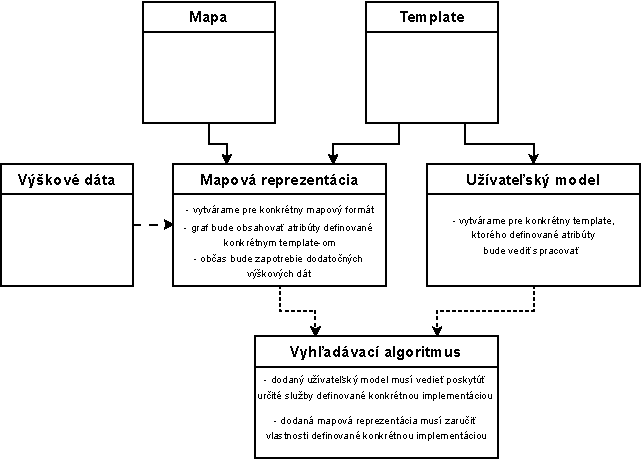
\includegraphics[]{img/konceptove_zavislosti}
\caption{Diagram závislostí jednotlivých konceptov} 
\label{obr01:konceptove_zavislosti}
\end{figure}

\pagebreak

\section{Zvolené implementačné prostriedky}

\subsection{Použitý programovací jazyk}

Pre implementáciu aplikácie bol vybraný jazyk C\#. Jazyk bol vybraný pre jeho jednoduchosť a bezpečnosť použitia. Alternatívnou volbou by mohol byť jazyk Java, ktorý má blízko práve ku C\#. Jeho nedostatočná znalosť v dobe začiatku práce ho však vyradila z použiteľných možností. 

Ďalšími možnosťami by mohol byť typicky vysoko-úrovňový jazyk Python alebo nízko úrovňový jazyk C++. Nakoľko v aplikácii bude prebiehať mnoho výpočtov, python by nebol vhodnou voľbou pre nedostatočnú rýchlosť ním vytvoreného strojového kódu. Na druhú stranu, C++ by bol dobrým kandidátom z hladiska výpočtovej sily. V tomto prípade však narážame opäť na nie veľmi dobrú znalosť tohto jazyka a na jeho programátorskú neprívetivosť. Pri väčšom projekte sme považovali za potrebné mať istotu, že nás použitý jazyk v programovaní podrží. 

Vhodnou úpravou implementácie by bolo implementovať výpočtovo náročné procesy v jazyku typu C++ a následne túto implementáciu volať externe z C\# jadra.     

\subsection{Užívateľské rozhranie}

Pre implementáciu užívateľského rozhrania som sa rozhodol pre \textit{Avalonia UI} framework. Užívateľské rozhranie je veľmi jednoduché. Bolo vytvorené tak, aby zabezpečilo všetku funkcionalitu.

V C\# existuje viacero možných knižníc, z ktorých bolo možné si vybrať:
\begin{itemize}
    \item GUI knižnice, ktoré sú súčasťou samotného .NET framework-u:
    \begin{itemize}
        \item \textbf{Windows Forms} je klasická GUI knižnica. Je jednoducho použiteľná a vďaka jej dlhoročnej podpore aj robustná a spoľahlivá. Jej vek je však aj jej nevýhodou, nakoľko vzhľad aplikácií vytvorených za pomoci Windows Forms príde človeku pomerne zastaralý. Ďalšou nevýhodou je rastrová povaha jeho renderovcieho engine-u. Táto vlastnosť sa nehodí pre aplikáciu, ktorej jedným z hlavných účelov je vykreslovanie mapových, vektorových objektov.     
        \item \textbf{Windows Presentation Foundation (WPF)} je modernejší nástupca Windows Forms. Aplikácie tvorené touto knižnicou majú modernejší vzhľad a sú generované renderovacím enginom založeným na vektorovej grafike. Ku programovaniu sa tu využíva popri C\# aj XAML, v ktorom sa definuje layout užívateľského rozhrania. Avšak spoločne s Windows Forms je ich spoločnou nevýhodou platformová závislosť na operačnom systéme Windows.
        \item \textbf{.NET MAUI} je nástupcom \textit{Xamarin.Forms}. Je to open-source-ový cross-platformný framework s množinou UI nástrojových balíčkov pre jednotlivé platformy. Podobne ako vo WPF sa pre vytváranie UI využíva kombinácia C\# a XAML. 
    \end{itemize}
    \item Alternatívou ku vstavaným .NET GUI knižniciam je práve nezávislá, open-source knižnica \textbf{Avalonia UI}. Čo do vlastností je veľmi dobre porovnateľná s \textit{.NET MAUI}. Hlavný rozdiel medzi týmito dvomi knižnicami je v~spôsobe, akým vykresľujú užívateľské rozhranie. Avalonia zapojuje kresliaci engine poháňaný knižnicou pre 2D grafiku \textit{Skia}. Na druhú stranu MAUI využíva natívne nástrojové balíčky pre každú platformu zvlášť. Ďalším rozdielom je, že Avalonia, na rozdiel od MAUI, podporuje aj niektoré distribúcie Linuxových systémov.
\end{itemize}

Rozhodnutie nakoniec padlo na využitie framework-u Avalonia UI. Nakoľko je veľmi podobný natívnemu .NET MAUI, rozhodla podpora pre Linuxové systémy a aj kvalitne spravená dokumentácia, z ktorej sa ľahko dalo vyčítať, ako sa s knižnicou má pracovať. 

Informované rozhodnutie pre výber GUI knižnice bolo učinené na základe zdrojov \cite{WpfGuide,WhatIsMAUI,AvaloniaMauiComparison}. Zároveň väčšinu informácií, ktoré som o Avalonia UI počas tvorby programu čerpal, pochádzali z jej dokumentácie \cite{AvaloniaDokumentacia}.

\subsection{Architektúra Model-View-ViewModel (MVVM)}\label{ArchitekturaMVVM}

Jeden z ďalších dôležitých aspektov, ktorý hral úlohu vo výbere knižnice pre užívateľské rozhranie, bola podpora \textit{MVVM} návrhového vzoru. Dokumentácia Avalonia UI popisuje architektúru MVVM následovne: \uv{The Model-View-View Model (MVVM) pattern is a common way of structuring a UI application. It uses a data binding system that helps move data between its view and view model parts. This means it achieves separation of application logic (view model) from the display of the UI (view). Separation between the application logic and the business services (model) is commonly achieved by a Dependency Injection (DI) system.}\cite{MVVMDefByAvalonia}.

MVVM architektúra je vhodná pre našu aplikáciu, nakoľko pre jej rozsah by klasická \textit{event-driven code-behind} architektúra nemusela postačovať. Týmto spôsobom zaručíme lepšiu separáciu a dostatočnú vnútornú nezávislosť kódu.    

V našej aplikácii bude tento návrhový vzor uplatnený s jemnou obmenou. Vrstva View model, ktorá v pôvodnom návrhovom vzore zastávala úlohu logiky aplikácie, bude rozdelená na dve časti: View model a novo vzniknutý \textit{Model view}. Viac informácií o tejto úprave je možné nájsť v sekcii \ref{MVVMNavrhovyVzor}. 

\subsection{Reaktívne programovanie}

Ďalším dôležitým aspektom aplikácie je Avaloniou a architektúrou MVVM iniciované využitie \textit{reaktívneho programovania.} Avalonia pre aplikáciu tohto paradigma využíva framework \textbf{Reactive UI}. 

Tento framework definuje reaktívne programovanie ako \uv{Reactive programming is programming with asynchronous data streams.} a dodáva \uv{Event buses or your typical click events are really an asynchronous event stream, on which you can observe and do some side effects. Reactive programming is that idea on steroids. You are able to create data streams of anything, not just from click and hover events. Streams are cheap and ubiquitous and anything can be a stream: variables, user inputs, properties, caches, data structures, etc.}\cite{ReactiveProgrammingByReactiveUI}.

V aplikácii sa bude tento framework využívať prevažne vo vrstvách View a View model, medzi ktorými prebieha väčšina reaktívnej komunikácie. 
\chapter{Architektúra ako celok}

Architektúra aplikácie má mriežkovú štruktúru. Je tvorená horizontálnymi (MVVM návrhový vzor) a vertikálnymi (\textit{session}-y + hlavné okno) vrstvami. V následujúcich sekciách popíšeme, ako jednotlivé vrstvy vyzerajú, aké su ich úlohy a ako medzi sebou komunikujú. Na konci kapitoly je následne k nahliadnutiu diagram \ref{obr02:priklad_struktury} znázorňujúci príklad možnej architektúry aplikácie.   

\section{MVVM(MV) návrhový vzor}\label{MVVMNavrhovyVzor}

Ako už bolo spomenuté v podsekcii \ref{ArchitekturaMVVM}, v aplikácii je využívaný návrhový vzor MVVM s drobnou obmenou. Táto obmena sa týka rozdelenia originálnej vrstvy View model do dvoch častí: View model a Model view. Toto rozdelenie zaručí ešte o niečo lepšiu separáciu kódu a odľahčí tým úlohy View model vrstvy. 

MVVM(MV) architektúra teda rozdeluje aplikáciu na 4 vrstvy: View, ViewModel, ModelView a Model. Popis jednotlivých vrstiev je k nahliadnutiu v následujúcich podsekciách. 

\subsection{View}

View je vrstva, ktorá popisuje a implementuje grafickú stránku aplikácie a určuje, akým spôsobom sa dáta dodané vrstvou View model zobrazia užívateľovi. View-y sú objekty viazané na odpovedajúce view model-y za pomoci reaktívneho programovania. Spracovávajú akcie užívateľa a iniciujú reakcie zvyšných vrstiev architektúry prostredníctvom príslušného view model-u. Následne zabezpečujú zobrazovanie dodaných výsledkov reakcie.

View vrstva je implementovaná za pomoci Avalonia UI framework-u. V náväznosti na tento fakt sú v aplikácii použité tri hlavné typy view-ov:
\begin{itemize}
    \item \textbf{Window} - Reprezentujú špecifické okná aplikácie, \uv{top-level} kontajnery, ktoré v sebe držia nejaký obsah. Okná sami o sebe nedefinujú vzhľad aplikácie. Slúžia predovšetkým ako rám, v ktorom sa striedajú jednotlivé view-y. Každé okno má naviazaný svoj vlastný view model, ktorý drží informáciu o tom, aký view je v danej chvíli v okne zobrazovaný. Naviazaný view model taktiež obsahuje vlastnosti, ktoré priamo súvisia s vlastnosťami daného okna.
    \item \textbf{View} - Sú to hlavné zložky, ktoré nesú grafiku zobrazujúcu sa oknách. Reprezentujú \uv{pohľady}, ktoré sú užívateľovi vykresľované. Každý view je naviazaný na špecifický view model. Viaže sa na jeho vlastnosti a reaktívne vykresluje dáta, ktoré tieto vlastnosti nadobúdajú. 
    
    Býva zvykom že sa konkrétny view zobrazuje práve v jednom konkrétnom okne. V takom prípade si na jeho view model drží referenciu view model daného okna. Za pomoci tejto referencie potom dokáže oknu jeho view model oznámiť, že sa v ňom má daný view zobraziť. 
    \item \textbf{DataTemplate} - Definuje grafickú reprezentáciu dát dodávaných z View model vrstvy do vrstvy View. Pre každý dátový typ, ktorý chce byť správne vykreslený pre užívateľa, musí existovať špecifický dátový template, pomocou ktorého sa daný údaj vykreslí. Dátové template-y sú špecifické tým, že sú raz definované pre celú aplikáciu, aby sa zachovala konzistencia vykreslovania jednotlivých dátových typov.
    
    Je potrebné podotknúť, že na to aby údaj vygenerovaný vo vrstve Model bolo možné vykresliť, musí preňho najprv existovať tzv. \textit{data view model} do ktorého sú jeho informácie zabalené a až v takejto podobe predávané nejakému view model-u, ktorý ich následne pomocou svojich vlastností odovzdá view-u na vykreslenie. Pre každý dátový view model sa následne hľadá príslušný DataTemplate, pomocu ktorého v ňom držané informácie zobrazia užívateľovi. 
\end{itemize}   

View vrstva je implementovaná pomocou dvoch jazykov: C\# a XAML. Pomocu XAML definujeme všetky polohy a tvary grafických objektov a bind-ujeme vlastnosti týchto objektov na vlastnosti z vrstvy View model. Pre každý view máme obecne jeden špecifický XAML súbor ktorým ho implementujeme. Ku väčšine XAML súborov je priradený C\# zdrojový súbor v ktorom sa implementuje takzvaný \textit{code-behind}. V tomto zdrojovom súbore môžeme doplniť všetku funkcionalitu view-u, ktorú nebolo možné vyjadriť jazykom XAML.    

\subsection{View model}\label{ViewModel}

Druhou v poradí je vrstva View model. Táto vrstva je zodpovedná za logiku spracovania akcií užívateľa oznámených reaktívnym spôsobom View vrstvou. Disponuje vedomím toho, aké akcie a v akom poradí sa majú vykonať pre zabezpečenie správnej reakcie na detegovaný impulz. K tomuto účelu využíva služby nižších vrstiev prostredníctvom volania metód na vrstve Model view. Tá na základe svojej vnútornej logiky vráti odpoveď s požadovanými údajmi. View model následne spracuje dodané dáta a predostrie ich vrstve View, aby ich mohla zobraziť užívateľovi.

View model na základe aplikačnej logiky koriguje a obmedzuje akcie užívateľa a tým zabraňuje vzniku nekonzistentných stavov aplikácie. Taktiež v niektorých prípadoch iniciuje \textit{interakcie} s inými view model-mi za účelom získania ich doplňujúcich služieb do jeho vlastného procesu.


Podobne ako vo View vrstve sa view model-y delia na tri základné typy:
\begin{itemize}
    \item \textbf{Session view model} + \textit{Main window view model} - Odpovedajú jednotlivým \textit{session}-om, ktoré sú základným kameňom vertikálnej štruktúry aplikácie. Viac informácií o session-och je možné nájsť v sekcii \ref{Sessions}. Výnimkou je práve \textit{Main window view model}, ktorý je naviazaný na hlavné okno aplikácie a zabezpečuje preň aplikačnú logiku. Klasické session view model-y sú taktiež naviazané zvyčajne na jedno okno z vrstvy View, pre ktoré zabezpečujú aplikačnú logiku.
    
    Každý session view model obsahuje kolekciu príslušných view model-ov, ktoré spoločne implementujú mechanizmus daného session-u. Je zvykom, že v jednej chvíli je aktívny iba jeden view model. O aktívnom view model-e je informované okno viazané na daný session view model. To následne v sebe zobrazuje odpovedajúci view aktívneho view model-u. Informovanie o aktívnom view model-e je hlavnou pracovnou náplňou session view model-u.

    K ďalším jeho povinnostiam patrí spracovávanie užívateľom vyvolaných akcií, ktoré sa týkajú samotného naviazaného okna. Príkladom takej akcie môže byť požiadavka o zatvorenie dotyčného okna.
    \item \textbf{View model} - Reprezentujú zložky, ktorých funkcionalita sa najväčšmi ponáša na obecnú, vyššie popísanú funkcionalitu vrstvy View model. Väčšina view model-ov spadá pod réžiu konkrétneho session-u (alebo hlavného okna), pre ktorý implementuje určitú časť jeho mechanizmu. Klasicky sú view model-y naviazané na príslušné view-y z vrstvy View. S tými následne reaktívne komunikujú a reagujú na ich podnety. View model-y sú navzájom nezávislé. To znamená, že medzi nimi neprebieha takmer žiadna komunikácia ani presun dát. Túto funkciu na seba berie Model view vrstva.

    Väčšina view model-ov by mala byť zahrnutá v zodpovedajúcom session view model-e (poprípade Main window view model-e). Ten potom zabezpečuje správu toho, ktorý view model je v danej chvíli aktívny. 
    
    Výnimkou sú view model-y, ktoré sú výhradne používane pre interakcie z iných view model-ov, ktorým týmto spôsobom doručujú svoje služby. Tieto view model-y sú väčšinou vytvorené na mieste interakcie a po jej skončení zanikajú. Pri ich vytváraní im sú zvyčajne predané nejaké vstupné parametre a keď je ich práca dokončená, vracajú jej výsledok. 
    \item \textbf{Data view model} - slúžia ako kontajnery pre informácie abstrahované z dát vygenerovaných v Model vrstve. Dáta sú klasicky konvertované do ich zodpovedajúcich view model-ov v Model view vrstve a už takto zabalené informácie sú predávané do View model vrstvy, kde sú spracované a pomocou vlastností odovzdané vrstve View na zobrazenie. Data view model-y môžu dodané informácie drobne upravovať takým spôsobom, aby ich bolo jednoduchšie zobrazovať vo View vrstve.
    
    Z toho vyplýva, že na to, aby nejaký údaj vygenerovaný v Model vrstve mohol byť prezentovaný užívateľovi, musí preňho existovať odpovedajúci data view model. Zároveň na to, aby informácie obsiahnuté v dátovom view model-e mohli byť vykreslené pre užívateľa, musí vo View vrstve existovať zodpovedajúci \textit{dátový template}, ktorý sa postará o ich správne grafické znázornenie.

    Niektoré data view model-y nielen že obsahujú informácie príslušných dát, ale obsahujú aj dáta samotné. Takéto data view model-y označujeme pomocou slova \textit{wrapping}. (tvoria akýsi obal okolo daných objektov). Táto funkcionalita je dôležitá hlavne v prípadoch, kedy data view model slúži taktiež pre spätnú komunikáciu s Model view vrstvou. V takých prípadoch musí byť možné identifikovať, ktorú dátovú inštanciu \uv{obaluje}. Wrapping data view model-y sú stotožnené s ich dátovým objektom a tiež sa pomocou neho identifikujú.  
\end{itemize}


View model je prvá z vrstiev, ktorá je kompletne písaná v jazyku C\#. Komunikácia medzi View model a View vrstvami funguje čisto na báze reaktívneho programovania za pomoci štruktúr z \textit{Reactive UI} framework-u.  

\subsection{Model view}

Treťou v poradí je, do klasickej MVVM architektúry pridaná, Model view vrstva. Táto vrstva je zodpovedná za \uv{vnútornú} logiku aplikácie. Priamo komunikuje s Model vrstvou a využíva jej zdroje pre zabezpečenie svojich služieb pre View model vrstvu. Dá sa povedať, že nedisponuje vlastným \uv{vedomím}. Medzi jej hlavné úlohy patria:  
\begin{itemize}
    \item prijímanie a spracovávanie požiadaviek od vrstvy View model a dodávanie očakávaných výsledkov.  
    \item zabezpečovať \textit{vnútro-session-ovú} komunikáciu. Model view-y v rámci jedného session-u si na seba držia referencie a predávajú si medzi sebou držané dáta. Táto komunikácia by mala byť vyšším vrstvam skrytá a na povrch by mal byť vidieť iba interface, pomocou ktorého prebieha komunikácia s View model-om.
    \item konverzia dát, získaných od Model vrstvy, do odpovedajúcich data view model-ov pri ich posielaní do vyšších vrstiev.  
\end{itemize}
Na druhú stranu medzi jej povinnosti nepatrí kontrola konzistentnosti jej vlastného stavu. O konzistenciu stavu aplikácie sa má starať View model.

V aplikácii používame model view-y dvoch typov:
\begin{itemize}
    \item \textbf{Session model view} + \textit{Main window model view}  - Odpovedajú jednotlivým session-om. (Viac informácií o session-och je možné nájsť v sekcii \ref{Sessions}). Ich hlavnou úlohou je vytvoriť a distribuovať model view-y odpovedajúce danému session-u. Pri ich inicializácii sa medzi model view-mi vytvoria väzby, ktoré sú následne počas behu aplikácie využívané na spomínanú vnútro-session-ovú komunikáciu. 
    
    Ďalej zabezpečujú spracovávanie požiadaviek pre odpovedajúce session view model-y. Tieto požiadavky sa typicky týkajú akcií, ktoré súvisia so session-om ako takým. Môže sa jednať napríklad o reakcie na zatváranie odpovedajúceho session-ového okna.  
    
    Výnimkou je práve \textit{main window model view}, ktorý je viazaný na view model hlavného okna a spracováva jeho požiadavky. V ostatných aspektoch je ale identický s klasickým session model view-om.
    
    Každému session model view-u odpovedá jeden konkrétny session view model. Ten pri svojej inicializácii predá model view-y, dodané v session model view-e, svojím odpovedajúcim view model-om.   
    \item \textbf{Model view} - typ, ktorý nesie vyššie popísanú funkcionalitu Model view vrstvy. Zvyčajne pre každý view model existuje dedikovaný model view, ktorý sa stará o zabezpečenie view model-om požadovaných služieb. Nie je to však pravidlo, view model môže obsahovať odkazy na viacero model view-ov, ktorých služby následne využíva alebo sú predané novo vytvoreným, v interakciách využívaným, view model-om.

    Je zvykom, že každý model view spadá pod nejaký konkrétny session alebo hlavné okno. V takom prípade je daný model view vytváraný a distribuovaný odpovedajúcim session model view-om/main window model view-om.  
\end{itemize}

\subsection{Model}\label{model}

Poslednou \uv{horizontálnou} vrstvou je Model. Je zodpovedná za doručovanie dát vyšším vrstvám a za doručenie mechanizmov pracujúcich s týmito dátami. Model sa svojou štruktúrou diametrálne odlišuje od predchádzajúcich vrstiev. Je tvorený jednotlivými oblasťami, ktoré spravujú dedikovaní \textit{manažéri}. Manažéri sú pristupovaný z jednotlivých model view-ov a doručujú im svoje služby, či už informatívne alebo výpočtové. Predstavujú interface-y ponúkajúce prívetivejší spôsob práce s vnútornými mechanizmami model-ov. 

Model je predstaviteľom jedinej perzistentnej \uv{horizontálnej} vrstvy. Manažéri sú väčšinou singleton triedy, ktoré ponúkajú služby všetkým session-om počas celej doby behu aplikácie. Vďaka tomuto spôsobu obsluhy je Model jediná vrstva, ktorej oblasti niesu viazané na žiadnu vertikálnu vrstvu (session/hlavné okno). Z návrhu Model vrstvy vyplýva, že model-y musia byť schopné svoje služby dodávať paralelne pre viacero session-ov naraz. 

Model vrstva je jednoducho rozšíriteľná o nové oblasti. Vďaka \textit{singleton} štruktúre sú oblastní manažéri dosiahnuteľní v podstate z akéhokoľvek miesta v programe a teda nemusia byť nikde zahrnutí. Manažéri by nemali mať problém prijímať nové, primerane vytvorené implementácie typov mechanizmov a dát z ich oblastí. Napríklad by nemalo byť zložité dodať nový vyhľadávací algoritmus odpovedajúcemu manažérovi, ktorý ho následne bude ponúkať zvyšku aplikácie. Viac informácií o návrhu architektúry jednotlivých oblastí vrstvy Model je možné nájsť v kapitole \ref{architektura_model_vrstvy}.

Špecifickým znakom komunikácie medzi Model a Model view vrstvami je ten, že pri nej dochádza ku strate typovej informácie dodávaných dát. Táto vlastnosť je motivovaná jednoduchým faktom, ktorým je udržanie vrstvy Model view jednoduchou. V Model vrstve sa totiž vo veľkom využívajú generiká pre jednoduché prenášanie typovej informácie v ich mechanizmoch. 

Využívanie generických typov v Model view vrstve by však prinieslo značné komplikácie v jej implementácii a tomu odpovedajúce zneprehladnenie kódu. Už len Model samotný trpí jemnou, generikami spôsobenou neprehľadnosťou. Z tohto dôvodu bolo rozhodnuté zabezpečiť jednoduchosť vrstvy Model view za cenu straty typovej informácie dát tečúcich z model-ov do model view-ov. 

Pri opačnom smere komunikácie je manažérmi typová informácia dodaných parametrov opäť testovaná a získavaná (väčšinou za pomoci tzv. \textit{generic visitor pattern}. Viac informácii o tejto modifikácii klasického \textit{visitor pattern} návrhového vzoru nájdete v kapitole \ref{architektura_model_vrstvy}.

Vo vrstve Model existujú popri manažéroch ešte aj tzv. \textit{sub-manažéri}. Tieto entity sú ale určené pre využitie z vrstvy Model. Podporujú generickú komunikáciu, na ktorej báze model-y fungujú, bez straty typovej informácie a teda sú príjemnejšie pre model-ovú komunikáciu než klasickí manažéri.     

\section{Session-y + \textit{hlavné okno}}\label{sessions_hlavne_okno}

\subsection{Session-y}

Aplikácia, či už z vizuálneho, logického alebo implementačného hladiska, je rozdelená do tzv. \textit{session}-ov. Session-y sú najväčšie stavebné jednotky, z ktorých každá predstavuje jedinečný mechanizmus dodávaný aplikáciou. Existencia ich inštancií je pominuteľná - vznikajú a zanikajú na popud užívateľa. Session-ov (aj rovnakého druhu) môže byť v aplikácii spustených viacero naraz. Každý session je klasicky tvorený odpovedajúcimi objektmi z prvých troch vrstiev horizontálnej štruktúry. 

Dodatočne môžu session-y využívať cudzie objekty z prvých troch vrstiev horizontálnej štruktúry, ktoré patria buď hlavnému oknu alebo inému typu session-u. V takom prípade by malo byť ale poriadne rozmyslené, či takéto \uv{postranné} využitie dáva zmysel a či sa ním neporušujú zasady používania daného view-u, view model-u alebo model view-u. 

Poprípade je možné využívať špecifické model view-y a view model-y prostredníctvom \textit{interakcií}. V takom prípade by ale dané objekty mali byť na daný účel prispôsobené (viac info v podsekcii \ref{ViewModel}, bod \textbf{View model}, 3. odsek).

Session-y sú klasicky rozdelené na logické časti, ktoré spolupracujú na dodaní požadovaného mechanizmu. Môžu napríklad reprezentovať konkrétne fázy jeho procesu. Každá časť je väčšinou tvorená jednou triedou z každej vrstvy View, View model a Model view.  %Tieto časti sú väčšinou tvorené špecifickými objektmi naprieč prvými tromi vrstvami horizontálnej štruktúry.

Jednotlivé session-y by medzi sebou nemali navzájom komunikovať ani zdielať svoje dáta. Mohlo by to viesť ku problémom s paralelizáciou služieb vykonávaných vrstvou Model.

Session-y ako také reprezentujú cestu ku všeobecnej rozšíriteľnosti aplikácie o novú aplikačnú logiku. Ak by vznikla potreba, aby aplikácia obsahovala nejaký nový mechanizmus, stačí preňho vytvoriť odpovedajúci session a upraviť hlavné okno tak, aby ho vedelo ponúknuť užívateľovi.  

\subsection{Hlavné okno}\label{Hlavne_okno_obecne}

Session-y sú vytvárané a spravované takzvaným \textit{hlavným oknom}. Je to jediná perzistentná \uv{vertikálna} vrstva aplikácie. Beh aplikácie začína otvorením tohto okna a končí jeho zatvorením. Hlavné okno môže byť používané počas celého behu aplikácie. Pokiaľ je vydaný pokyn na uzavretie hlavného okna, pričom sú stále živé niektoré session-y, užívateľ môže byť na tento fakt upozornený. Ak mu to ale neprekáža, zatvorením hlavného okna sa zavrú aj všetky ostatné a aplikácia sa ukončí. Logika session-ov by mala túto skutočnosť brať do úvahy.

Horizontálna štruktúra hlavného okna je veľmi podobná tej session-ovej. Taktiež využíva MVVM(MV) architektúru. Jej časti sú ale z podstaty hlavného okna vytvárané len raz pri štarte aplikácie a zanikajú pri jej ukončení. \textit{Session view model} a \textit{Session model view} sú nahradené za funkčne identické \textit{Main window view model} a \textit{Main window model view}. Podobne ako pri session-och, aj hlavné okno je rozdelené do niekoľkých častí. Tie si medzi sebou rozdeľujú jeho funkcionalitu. Niektoré z jeho častí môžu byť sprístupnené rôznym session-om, aby si z nich mohli vytiahnuť potrebné parametre platiace pre celú aplikáciu.     

Ako bolo spomenuté na začiatku tejto podsekcie, hlavné okno vytvára, eviduje a spravuje inštancie všetkých session-ov. Definuje maximálny počet aktívnych session-ov, spravuje session-y pri ukončovaní aplikácie, poskytuje \textit{dodávateľa} hlavných parametrov, inicializuje pri vytváraní session-u jeho session view model a session model view.  

\begin{figure}[p]\centering
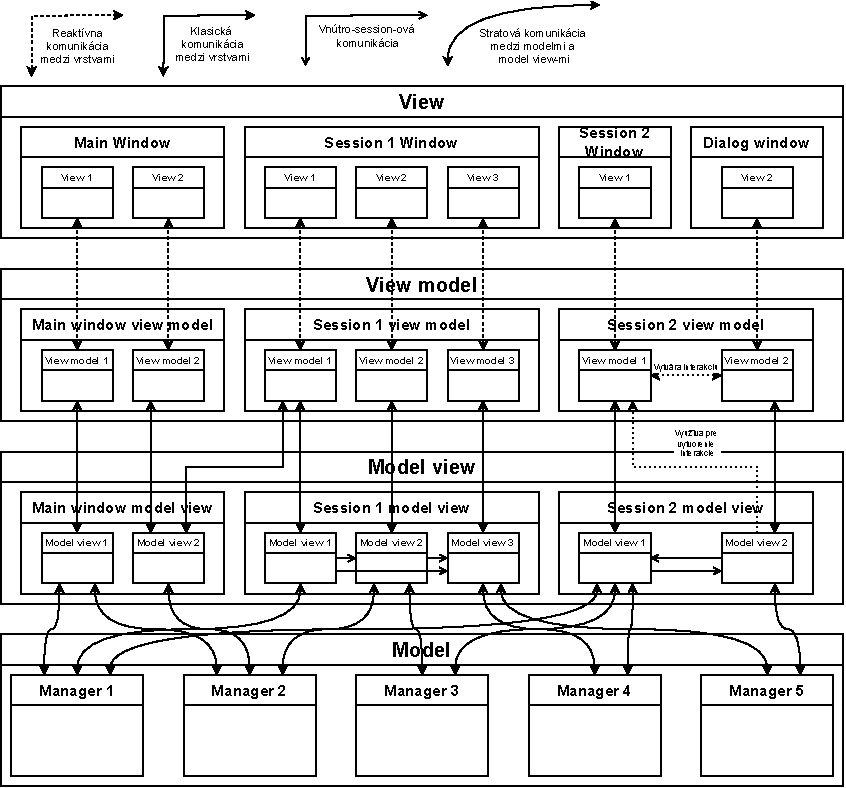
\includegraphics[]{img/priklad_struktury}
\caption{Príklad možnej \uv{mriežkovej} štruktúry aplikácie.} 
\label{obr02:priklad_struktury}
\end{figure}

\chapter{Vertikálna štruktúra aplikácie}

V~tejto kapitole uvádzame bližší pohľad na~súčasnú podobu hlavného okna a~session-ov aplikácie. Aktuálne aplikácia disponuje len jedným typom session-u určeným pre~samotné vyhľadávanie ciest v~mapách (\textit{Path finding session}). Viac informácií o~vertikálnej štruktúre aplikácie je možné nájsť v~Sekcii~\ref{sessions_hlavne_okno}.

\section{Hlavné okno}

O obecných úlohách hlavného okne sme sa zmienili už v~Podsekcii~\ref{Hlavne_okno_obecne}. V~tejto sekcii sa pozrieme na~aktuálne implementovanú architektúru, ako aj~funkcionalitu hlavného okna.


Hlavné okno je tvorené dvomi časťami: hlavným menu a~hlavnými nastaveniami.
Popri tom interaktívne využíva v~nastaveniach služby mechanizmu pre~správu výškových dát.

Ako už bolo spomenuté v~Podsekcii~\ref{Hlavne_okno_obecne}, po~zatvorení hlavného okna sa ukončuje aj~aplikácia. Tým pádom je úlohou hlavného okna zaistiť uloženie všetkých parametrov aplikácie pre~využitie v~budúcich behoch.

V~následujúcich podsekciách popíšeme časti, z~ktorých je aktuálne hlavné okno tvorené. Na~konci tejto sekcie je zobrazený Diagram~\ref{obr03:hlavne_okno} reprezentujúci jeho architektúru.

\subsection{Hlavné menu}

Hlavné menu je prvá časť, ktorá sa v~hlavnom okne užívateľovi po~zapnutí aplikácie zobrazí. Obsahuje možnosti vytvorenia inštancií session-ov a~možnosť otvorenia hlavných nastavení aplikácie. 

View model hlavného menu si vedie evidenciu všetkých otvorených session-ov. Pri~detekcii zatvorenia hlavného okna sa stará o~ich správne ukončenie. Taktiež si drží referenciu na~sprostredkovateľa hlavných nastavení. Toho následne môže predať session-om, ktorý~ho môžu použiť pre~získanie parametrov platných pre~celú aplikáciu.

Zvláštnosťou tejto časti je absencia vlastného model view-u. V~aktuálnej podobe aplikácie totiž nie je potrebný, nakoľko hlavné menu nepotrebuje komunikovať so~žiadnym modelom ani inou časťou hlavného okna. Ak by táto potreba v~budúcnosti vznikla, nemal by byť problém model view pre~hlavné menu vytvoriť. 

Možné vylepšenie tejto časti by mohlo zahrňovať vypísanie všetkých aktuálne otvorených session-ov pre~užívateľa. Zaistilo by to preňho jednoduchšiu orientáciu v~aplikácii.

\subsection{Hlavné nastavenia}

Hlavné nastavenia sú druhou časťou hlavného okna. Zabezpečujú možnosť pre~užívateľa nastaviť parametre, ktoré~sú využívané celou aplikáciou. 

V~aktuálnom stave sú to len dve možnosti konfigurácie: možnosť zmeny lokalizácie aplikácie a~možnosť nastavenia implicitne používaného zdroja výškových dát (presnejšie konkrétnej distribúcie výškových dát daného zdroja). 

Lokalizácia je implementovaná na~základe lokalizačných .resx zdrojových súborov. Avalonia je schopná takéto zdroje využívať aj~na~zmenu pevných nápisov aplikácie. %Ak nestihnem prelozit aplikaciu, tak to tu spomenut...ze z~casovych dovodov

Zdroj výškových dát je nastavovaný za~pomoci interakcie s~mechanizmom konfigurácie výškových dát. Po~stlačení príslušného tlačidla sa v~hlavnom okne zobrazí view zodpovedajúci tomuto mechanizmu. Užívateľ si v~ňom môže vybrať, ktorú distribúciu dát chce implicitne v~aplikácii využívať. Viac informácií ohľadom konfigurácie výškových dat nájdete v~následujúcej podsekcii.

Do budúcna sa počíta s~rozšírením hlavných nastavení do~takej miery, aby~sa z~nich dali konfigurovať aj~rôzne preferencie vo~vrstve Model. Pre~toto rozšírenie by sa však museli upraviť oblasti vrstvy Model, aby~tieto konfigurácie dokázali prijímať.

\subsection{Konfigurácia výškových dát}\label{konfiguracia_vyskovych_dat}

Konfigurácia výškových dát má špecifický spôsob využitia. Je určená na~to byť otváraná pomocou interakcie, vytvorenej inou časťou aplikácie. Jej hlavnou funkciou je dodávanie mechanizmu sťahovania a~mazania výškových dát, ktoré~je možné využiť ako dodatočný informačný zdroj pri~vytváraní mapových reprezentácií. 

Výškové dáta sú sťahované zo~špecifických zdrojov. Zdroje výškových dát môžu obsahovať viacero dátových distribúcií. Tie sa môžu líšiť v~kvalite, presnosti či~dostupnosti dodávaných výškových dát. 

Manipulácia s~dátami je vykonávaná po~oblastiach zvaných \textit{regióny}. Veľkosť a~tvar regiónov si každá distribúcia dát definuje sama. 

V~niektorých prípadoch zdroj výškových dát môže vyžadovať k~ich sprístupneniu autorizáciu užívateľa pomocou mena a~hesla. Táto autorizácia nemusí byť požadovaná pre~všetky jeho dátových distribúciach. V~prípade potreby autorizácie mechanizmus zabezpečuje možnosť užívateľovi dané údaje poskytnúť. Následne sa aplikácia pokúsi na~ich základe požadované dáta získať.   

Sťahovanie a~mazanie dát prebieha asynchrónne. Užívateľ je informovaný o~tom, ktoré~regióny su aktuálne stiahnuté, sťahované, neprítomné a~odstraňované. Viacero regiónov môže byť sťahovaných/odstraňovaných naraz, či~už z~jedného alebo~rôznych dátových zdrojov. Správne asynchrónne fungovanie manipulácie s~dátami zaručujú implementácie zdrojov výškových dát v~Model vrstve.

Špecifickou vlastnosťou konfigurácie výškových dát je možnosť ju používať súčasne z~viacerých miest v~aplikácii. Je navrhnutá tak, aby~zvládala korektne akceptovať pokyny z~mnohých interakcií naraz. Vďačí za~to návrhu model view-u, ktorý~poskytuje informácie o~tom, v~akom štádiu sťahovania sú jednotlivé regióny. Vďaka tomu všetky naviazané view model-y získajú aktuálne informácie a~môžu správne korigovať manipuláciu s~výškovými dátami.

Spôsob používania konfigurácie výškových dát je následovný:
\begin{itemize}
    \item Pri~inicializácii interakcie je novo vytvorenému view model-u(následne použitému v~interakcii) predaná aktuálne využívaná distribúcia výškových dát.
    \item Tá je v~konfigurácii nastavená ako aktuálne konfigurovaná a~ukázaná pomocou view-u užívateľovi.
    \item Následne prichádza fáza samotného konfigurovania výškových dát. Užívateľ môže:
    \begin{itemize}
        \item Zmeniť aktuálne konfigurovanú distribúciu výškových dát.
        \item Sťahovať a~odstraňovať výškové dáta aktuálne vybranej distribúcie. Tieto úkony sú uskutočňované na~základe regiónov, definovaných konfigurovanou distribúciou.
        \item Zadať autorizačné údaje pre~možnosť využitia dát zo~špecifických distribúcií, ktoré~autorizáciu vyžadujú. 
        \item Ukončiť konfiguračnú interakciu.
    \end{itemize} 
    \item Pri~ukončení interakcie sa posledne konfigurovaná distribúcia vráti ako novo zvolená na~používanie.
\end{itemize}

\begin{figure}[h]\centering
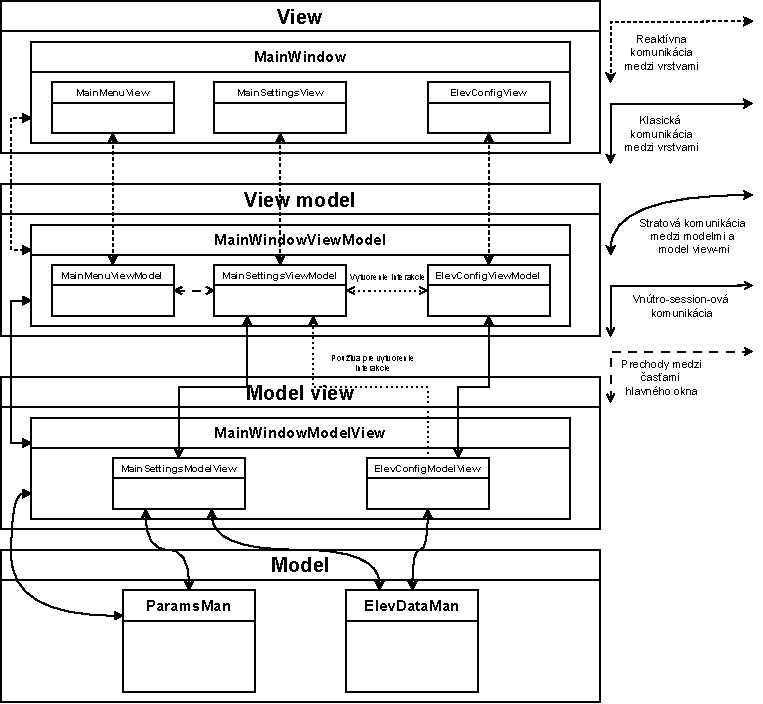
\includegraphics[]{img/hlavne_okno}
\caption{Diagram popisujúci architektúru hlavného okna aplikácie.} 
\label{obr03:hlavne_okno}
\end{figure}

\pagebreak

\section{Session pre~vyhľadávanie ciest v~mapách}

Vyhľadávanie ciest v~mapách je hlavnou náplňou aplikácie. V~tejto sekcii popíšeme typ session-u, ktorý~zabezpečuje logiku za~doručovaním tejto služby. Mechanizmus hľadania cesty v~mapách zahrnuje:
\begin{itemize}
    \item výber vstupných parametrov tak, aby~ich kombinácia bola platná, 
    \item vytvorenie grafickej reprezentácie mapy,
    \item vytvorenie mapovej reprezentácie, v~ktorej sa bude vyhľadávať cesta,   
    \item umožnenie užívateľovi zadať trať, na~ktorej sa má cesta vyhľadať,
    \item spustenie implementácie vybraného vyhľadávacieho algoritmu na~zvolenej trati a~vykreslenie nájdenej cesty. 
\end{itemize} 
V~aktuálnej podobe sa mechanizmus vyhľadávania cesty skladá z~troch častí: 
\begin{itemize}
    \item Nastavenie parametrov hľadania cesty (template, mapa, užívateľský model a~vyhľadávací algoritmus).
    \item Vytvorenie mapovej reprezentácie na~základe vybranej mapy a~template-u. Prípadne za~pomoci prítomných výškových dát. Táto časť je navrhnutá pre~použitie v~interakcii. Interakciu iniciuje časť nastavovania parametrov. 
    \item Spúšťanie zvoleného vyhľadávacieho algoritmu na~vytvorenej mapovej reprezentácii za~využitia výpočtov vybraného užívateľského modelu. Zahrňuje prijímanie trate od užívateľa a~vykreslovanie nájdenej cesty.
\end{itemize} 

Časť, ktorá sa z~časových dôvodov nedostala do~mechanizmu hľadania cesty je tzv. \textit{relevance-feedback} mechanizmus. Ten by slúžil pre~užívateľa na~dodatočné nastavenie hodnôt vybraného užívateľského modelu na~základe jeho preferencií vzhľadom k~aktuálne vybranej mape. Z~tejto časti zostal v~aplikácii len odpovedajúci model view, ktorý~v~tejto chvíli nenesie žiadnu užitočnú funkcionalitu. Slúži iba pre~prenos dát v~Model view vrstve. Bol v~aplikácii ponechaný z~dôvodu plánovaného budúceho rozšírenia aplikácie o~relevance-feedback mechanizmus.

V~následujúcich podsekciách popíšeme časti, z~ktorých je aktuálne session tvorený. Na~konci tejto sekcie je zobrazený Diagram~\ref{obr04:session_vyhladavania_cesty} reprezentujúci jeho architektúru.

\subsection{Nastavenia parametrov pre~vyhľadávanie cesty}

Nastavenia parametrov sú prvou časťou, ktorá je užívateľovi po~vytvorení session-u predostretá. Ten si za~jej pomoci zvolí:

\begin{itemize}
    \item template atribútov, ktoré~budú extrahované do~mapovej reprezentácie, 
    \item mapový súbor, na~základe ktorého sa bude vytvárať mapová reprezentácia. Teda súbor s~mapou, na~ktorej bude prebiehať vyhľadávanie ciest.
    \item súbor s~užívateľským modelom, ktorý~bude používaný algoritmom na~agregáciu hodnôt z~atribútov uložených v~mapovej reprezentácii  
    \item vyhľadávací algoritmus použitý na~hľadanie ciest v~mapovej reprezentácii za~pomoci výpočtov vybraného užívateľského modelu
\end{itemize}

Na začiatku sa predvolia parametre na~tie, ktoré~boli použité v~predchádzajúcej inštancii session-u. Uložené parametre prežívajú aj~samotné behy aplikácie.  

Vyberanie parametrov sa musí riadiť istými pravidlami z~dôvodu závislostí jednotlivých typov objektov, popísaných v~podsekciách Sekcie~\ref{Aspekty_hladania}. Danými pravidlami sú:
\begin{itemize}
    \item Jednotlivé parametre sa nastavujú postupne. Najprv je nutné, aby~bol vybraný mapový súbor a~template. Následne môže byť vybraný aj~súbor s~užívateľským modelom. Keď sú všetky tri predchádzajúce položky vybrané, je možné vybrať vyhľadávací algoritmus. 
    \item Pre~zvolenú kombináciu template-u a~formátu mapového súboru musí existovať mapová reprezentácia, ktorá túto kombináciu dokáže spracovať. Taktiež pre~zvolený template-u musí existovať typ užívateľského modelu, ktorý~dokáže spracovávať atribúty definované týmto template-om. Nakoniec musí existovať aspoň jedna kombinácia takto definovanej mapovej reprezentácie a~užívateľského modelu, ktorú dokáže využiť aspoň jedna implementácie ľubovoľného vyhľadávacieho algoritmu.   
    
    Keď je vybraný buďto template alebo~mapový súbor a~výber druhej položky by spôsobil neplatnú kombináciu, prvá položka sa opäť vynuluje. Možným vylepšením by bolo zabezpečenie indikácie platných kombinácií template-ov a~formátov mapových súborov.
    \item Súbor s~užívateľským modelom môže byť vybraný len takého typu, ktorý~dokáže spracovávať atribúty definované zvoleným template-om a~ktorý spolu s~ľubovoľnou mapovou reprezentáciou, ktorá dokáže spracovať aktuálne zvolenú kombináciu template-u a~mapového formátu, je použiteľnou kombináciou pre~aspoň jednu implementáciu nejakého vyhľadávacieho algoritmu. 
    \item Vyhľadávací algoritmus následne môže byť zvolený len taký, ktorý~dokáže využiť vybraný užívateľský model a~niektorú mapovú reprezentáciu, ktorú je možné vytvoriť z~vybraného template-u a~mapového súboru.
\end{itemize}    

Po výbere mapového súboru sa ihneď z~agregovanej mapy vytvorí jej grafická reprezentácia a~jej náhľad sa zobrazí užívateľovi.

Po dosadení všetkých parametrov môže užívateľ pokračovať do~ďalšej časti mechanizmu, ktorou je vytváranie mapovej reprezentácie. V~okamžiku prechodu do~tejto časti sa taktiež uložia aktuálne nastavené parametre, aby~mohli byť znovu použité ako predvolené v~následujúcich inštanciách session-u. 

Proces vytvárania mapovej reprezentácie je vykonaný za~pomoci interakcie z~parametre-nastavovacej časti. Na~základe jej výsledku sa následne buď presunieme v~mechanizme ďalej do~cestu-vyhľadávacej časti (úspešné vytvorenie) alebo~zostaneme v~nastaveniach.(neúspešné vytvorenie).  

\subsection{Vytváranie mapovej reprezentácie}

Vytváranie mapovej reprezentácie je akási prechodová časť medzi nastaveniami a~samotným vyhľadávaním ciest v~mape. Je prevedená za~pomoci interakcie iniciovanej v~nastaveniach, po~dosadení všetkých potrebných parametrov. Táto interakcia je spracovaná pomocou dialógového okna. Pomocou neho môže užívateľ pozorovať priebeh tvorby mapovej reprezentácie a~aktívne sa zapájať pri~riešení vzniknutých problémov.  

Priebeh tvorby mapovej reprezentácie je nasledovný:
\begin{itemize}
    \item Ihneď po~inicializácii tejto časti sa spustí proces kontroly podmienok tvorby mapovej reprezentácie. Aktuálne je využívaná iba kontrola prítomnosti potrebných výškových dát pri~procese tvorenia mapovej reprezentácie. (Táto kontrola zahrňuje aj~schopnosť mapy dodať informácie o~svojej pozícii a~rozlohe, ktoré~sú nevyhnutné pre~získanie odpovedajúcich výškových dát).
    
    Pokiaľ tvorená mapová reprezentácia indikuje potrebu výškových dát, skontroluje sa, či~sú odpovedajúce dáta prítomné. Pokiaľ dáta prítomné niesu alebo~mapa nie je schopná definovať svoju geografickú polohu/rozlohu, vytváranie mapovej reprezentácie zlyhá a~užívateľ sa môže vrátiť do~nastavení. 
    
    Do~budúcna je v~pláne umožniť užívateľovi riešenie problému nedostatku výškových dát za~pomoci interakcie s~konfiguráciou výškových dát. Viac informácii o~konfigurácii výškových dát je možné nájsť v~Podsekcii~\ref{konfiguracia_vyskovych_dat}.
    \item Pokiaľ kontrola podmienok dobehne úspešne, je automaticky spustený proces vytvárania mapovej reprezentácie. Tento proces môže trvať dlhšiu dobu a~teda je užívateľovi umožnené sledovať jeho vývoj alebo~ho dokonca prerušiť. Po~prerušení je užívateľ vrátený naspäť do~nastavení parametrov.
\end{itemize}

\subsection{Vyhľadávanie cesty v~mape}

Po úspešnom vytvorení mapovej reprezentácie sa môžeme presunúť k~samotnému vyhľadávaniu ciest v~mape. V~tejto chvíli máme k~dispozícii všetky potrebné dátové zdroje k~správnemu vykonávaniu tejto činnosti.

Na začiatku je vykreslená grafika mapy, ktorá bola vytvorená v~nastaveniach pri~výbere mapového súboru.

Kolobeh vyhľadávania je rozdelený do~troch fáz:
\begin{itemize}
    \item Prvou fázou je umožnenie výberu trate užívateľovi. Trať sa skladá z~postupností bodov, medzi ktorými je následne vyhľadávaná cesta. Užívateľ môže pridávať a~odoberať koncové body trate.
    \item Po~zadaní cesty prichádza na~rad fáza samotného vyhľadávanie cesty. Algoritmus má možnosť podávať správy o~postupe vyhľadávania, či~už pomocou textovej informácie alebo~grafického znázorňovania. Užívateľ mám možnosť proces vyhľadávania predčasne ukončiť. V~takom prípade sa kolobeh vráti do~prvej fázy výberu trate.
    \item Pokiaľ vyhľadávania cesty dobehne úspešne, príde na~rad tretia fáza, ktorou je vykreslenie nájdenej cesty. Zároveň sa po~strane môžu vypísať informácie o~nájdenej trase (napríklad jej dĺžka, prekonané prevýšenie, atď.). V~tejto fáze je užívateľovi umožnené interagovať s~nájdenými cestami (s takými, ktoré~takúto funkcionalitu zabezpečujú). Po~dokončení prezerania nájdenej cesty sa opäť vrátime do~prvej fázy výberu trate.  
\end{itemize}

Počas ktorejkoľvek fázy je užívateľ schopný približovať, odďalovať a~hýbať so~zobrazenou grafikou vyhľadávania.

\begin{figure}[h]\centering
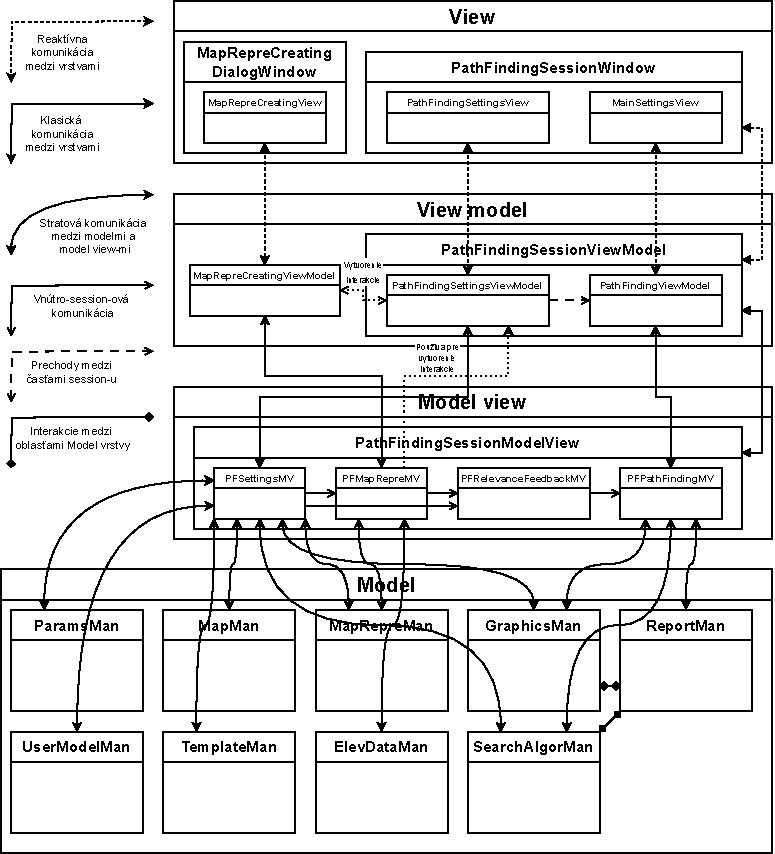
\includegraphics[]{img/session_vyhladavania_cesty}
\caption{Diagram popisujúci architektúru session-u pre~vyhľadávanie cesty v~mapách} 
\label{obr04:session_vyhladavania_cesty}
\end{figure}

% \subsection{Zaujímavé implementačné postupy} % % V~tejto podsekcii vymenujeme pár zaujímavých postupov využitých pri~implementácii \textit{hlavného okna}.  % \begin{itemize} % \item \textbf{Zatváranie hlavného okna} - zatváranie hlavného okna je špecifické tým, že~ukončuje beh celej aplikácie. Preto je v~niektorých prípadoch potrebné, aby~bolo možné sa opýtať užívateľa, či~si je istý svojou požiadavkou na~ukončenie aplikácie. Ideálnym spôsobom na~zistenie užívateľovho názoru je použitie dialógového okna. Ač sa to môže zdať ako triviálna úloha, s~Avalonia framework-om to zas tak jednoduché nebolo.  % % Následujúci kód ukazuje nefunkčný príklad \texttt{MainWindow\_OnClosing} metódy z~triedy \texttt{MainWindow} určenej na~zachytávanie a~spracovanie udalosti zatvárania hlavného okna: % % \begin{lstlisting} % private async void MainWindow_OnClosing % (object? sender, WindowClosingEventArgs e) % { % bool close = % await ViewModel!.OnClosingCommand.Execute(); % if (!close) % { % e.Cancel = true; % } % } % \end{lstlisting} % 
    % Na~prvý pohľad by sa mohlo zdať že~je všetko v~poriadku. Pokiaľ spustený \texttt{ViewModel.OnClosingCommand} vráti indikáciu toho, že~sa okno nesmie zavrieť, nastaví sa vlastnosť \texttt{Cancel} na~true a~tým sa zabráni zatvoreniu hlavného okna.
    % 
    % Problém je však v~tom, že~spustenie daného príkazu na~view modelu prebieha asynchrónne z~dôvodu možnosti otvorenia dialógového okna na~komunikáciu s~užívateľom. Výsledok príkazu je potrebné očakávať za~pomoci kľúčového slova \texttt{await}, nakoľko jeho použitie zabezpečí, že~UI thread zostane aktívne a~reagujúce.
    % 
    % To však na~druhú stranu sa stáva problémom, nakoľko UI spracuje argument \texttt{e} prv než naša metóda dokáže správne dosadiť jeho vlastnosť \texttt{Cancel}. Teda okno sa zavrie skorej, než je užívateľovi daná možnosť to zvrátiť.
    % 
    % Preto bol použitý následujúci návrh metódy, ktorý~zaručuje správny spôsob zatvárania hlavného okna:
    % \begin{lstlisting}
    % private bool _alreadyAsked = false;
    % private async void MainWindow_OnClosing
        % (object? sender, WindowClosingEventArgs e)
    % {
        % if (_alreadyAsked) return;
        % e.Cancel = true;
        % bool close = 
            % await ViewModel!.OnClosingCommand.Execute();
        % if (close)
        % {
            % _alreadyAsked = true;
            % Close();
        % }
    % }
    % \end{lstlisting}
% 
    % v~tomto prípade sme predošlý problém vyriešili malým trikom. Vždy keď zaznamenáme udalosť zatvárania okna iniciovanú užívateľom, nastavíme automaticky príznak \texttt{Cancel} argumentu \texttt{e} na~true. Tým zabránime predčasnému zatvoreniu okna. 
    % 
    % Následne podobne ako v~predošlom prípade asynchronne zavoláme spustenie \texttt{ViewModle.OnClosingCommand} a~počkáme na~výsledný indikátor. Ak indikuje pokračovanie v~zatváraní aplikácie, príde na~radu náš trik.  
% 
    % Nastavíme hodnotu, k~tomuto špecifickému účelu vytvoreného, privátneho poľa \texttt{\_alreadyAsked} na~true. Toto pole indikuje, že~sa hlavné okno už raz užívateľa pýtalo na~jeho názor na~zatvorenie aplikácie a~že jeho odpoveď bola pozitívna. 
    % 
    % Po~nastavení poľa je opäť zavolaná metóda Close() na~hlavnom okne. Na~základe tohto volania sa opäť hlavné okno pokúsi zavrieť. Tým pádom sa znova zavolá metóda \texttt{MainWindow\_OnClosing}. Tentokrát sa však jej beh zastaví hneď na~začiatku na~dotaze, či~pole \texttt{\_alreadyAsked} indikuje už zistený užívateľov súhlas so~zavretím okna. Tým pádom sa vlastnosť \texttt{Cancel} nestihne nastaviť na~true a~teda hlavné okno sa následne zavrie.    
% 
    % Tento princíp je možné využiť taktiež v~ostatných oknách aplikácie, ak by mali potrebu rovnakého mechanizmu ich zatvárania. 
    % \item \textbf{Súbežné využívanie inštancie \texttt{ElevDataModelView}-u} - za~možnosťou súbežného využívania model view-u konfigurácie výškových dát je malý trik. Na~začiatok je potrebné si uvedomiť, ktoré~dáta je potrebné držať synchrónne vo~všetkých používaných konfiguráciách výškových dát a~ktoré na~druhú stranu majú byť pre~každú konfiguráciu jedinečné:
    % \begin{itemize}
        % \item Synchrónne je potrebné držať informácie o~stave prítomnosti jednotlivých regiónov všetkých distribúcií. Keby sa v~týchto dátach objavila akákoľvek nesúmernosť, mohlo by to mať fatálne dôsledky na~manipuláciu s~výškovými dátami.
        % \item Na~druhú stranu každá konfigurácia by si mala sama určovať, ktorá distribúcia výškových dát je aktuálne konfigurovaná. Predsa len to je jedným zo~zámerov procesu konfigurácie. Nechať užívateľa vybrať ním žiadanú distribúciu na~použitie či~upravenie.
    % \end{itemize}
% 
    % Teda potrebujeme, aby~inštancia \texttt{ElevDataModelView} v~sebe držala informáciu o~prítomnosti jednotlivých regiónov pre~všetky distribúcie. Pre~konkrétny región je táto informácia uložená v~data view modele, do~ktorého je príslušný región zabalený (viac informácií k~data view modelom nájdete v~podsekcii~\ref{ViewModel}). Samotný región si nesie informáciu len o~tom, či~sú preňho dáta stiahnuté alebo~nie. Neinformuje ale~o~tom, čí sú dáta aktuálne sťahované alebo~odstraňované.
% 
    % Typicky model view-y vytvárajú vždy nový data view model pre~každý údaj získaný z~Model vrstvy v~momente posúvanie jeho informácie do~vrstvy View model. Tu však prichádza na~rad malý trik, kedy \texttt{ElevDataModelView} vytvorí data view modely pre~všetky existujúce regióny počas svojej inicializácie a~uloží ich do~slovníka \texttt{TopRegionsOfAllDistributions}. Následne je tento slovník ponúkaný všetkým inštanciám triedy \texttt{ElevConfigViewModel} a~teda všetky tieto inštancie pracujú s~jednými a~tými istými objektmi regiónových data view modelov.
    % 
    % Tým pádom všetky inštancie triedy \texttt{ElevConfigViewModel} zdieľajú informácie o~stave prítomnosti jednotlivých regiónov a~teda nemôže nastať nekonzistencia v~akciách manipulujúcich s~výškovými dátami. (samozrejme za~predpokladu, že~užívateľ nie je schopný stlačiť dve tlačidlá v~rôznych konfiguračných oknách v~ten istý moment. Pri~klasickom používaní aplikácie by tento scenár nikdy nemal nastať).
% 
    % Na~druhú stranu každá inštancia triedy \texttt{ElevConfigViewModel} si sama drží informáciu o~aktuálne konfigurovanej distribúcii výškových dát a~teda v~každej z~týchto inštancií môžem v~rovnakom čase konfigurovať inú distribúciu.
% \end{itemize}










% \subsection{Zaujímavé implementačné postupy}
% 
% v~tejto podsekcii vymenujeme pár zaujímavých postupov využitých pri~implementácii \textit{session-u pre~vyhľadávanie ciest v~mapách}.  
% 
% \begin{itemize}
    % \item \textbf{Spôsob zabezpečenia vnútornej komunikácie model view-ov} - Jednou z~náplní Model view vrstvy je zabezpečovať vnútro-session-ovú komunikáciu. Nikto okrem samotných model view-ov by nemal mať k~tejto komunikácii prístup. Okolie by mal mať možnosť vidieť iba metódy, ktorými Model view vrstva sprístupňuje svoje služby. 
    % 
    % Následujúca implementácia zaručuje ukrytie vnútornej komunikácie model view-ov cesty-vyhľadávacieho session-u. Môže slúžiť ako príklad pre~implementáciu Model view vrstvy ostatných session-ov. 
% 
    % Model view inštancie pre~daný session inicializuje \textit{session model view}. Ten ich následne aj~distribuuje do~ostatných potrebných častí session-u. 
    % 
    % Chyták však je, že~vytvárané inštancie niesu typu, ktorý~je navonok prezentovaný. Session model view definuje privátnych potomkov týchto prezentovaných typov, ktorí majú, narozdiel od ich predkov, implementovanú funkcionalitu vzájomnej komunikácie. Taktiež override-ujú všetku funkcionalitu predkov, v~ktorej je potrebná práca s~dátami prúdiacimi vo~vnútornej komunikácii.
% 
    % Tým že~sú tieto \uv{intra} triedy definované ako privátne, nie je možné mimo name-space-u session model view-u sledovať ich komunikáciu.
% 
    % \begin{listing}[h]
    % \begin{lstlisting}
    % public class PathFindingSessionModelView : SessionModelView
    % {
        % public PFSettingsMV Settings { get; }
        % public PFMapRepreCreatingMV MapRepreCreating { get; }
        % public PFRelevanceFeedbackMV RelevanceFeedback { get; }
        % public PFPathFindingMV PathFinding { get; }
        % 
        % public PathFindingSessionModelView()
        % {
            % var setI = new PFSettingsIntraMV();
            % var graCreI = new PFMapRepCreIntraMV(setI);
            % var relFeeI = 
                % new PFRelevanceFeedbackIntraMV(setI, graCreI);
            % var patFinI = new PFPathFindingIntraMV(relFeeI);
% 
            % Settings = setI;
            % MapRepreCreating = graCreI;
            % RelevanceFeedback = relFeeI;
            % PathFinding = patFinI;
        % }
        % private class PFSettingsIntraMV : PFSettingsMV        
        % private class PFMapRepreCreatingIntraMV : 
            % PFMapRepreCreatingMV
        % private class PFRelevanceFeedbackIntraMV : 
            % PFRelevanceFeedbackMV
        % private class PFPathFindingIntraMV : PFPathFindingMV
    % }
% 
    % public abstract class PFSettingsMV : ModelViewBase { }        
    % public abstract class PFMapRepreCreatingMV : 
        % ModelViewBase { }        
    % public abstract class PFRelevanceFeedbackMV : 
        % ModelViewBase { }
    % public abstract class PFPathFindingMV : ModelViewBase { }      
    % \end{lstlisting}
    % \caption{Príklad návrhu session model view-u, ktorý~skrýva vnútornú komunikáciu (upravený \texttt{PathFindingSessionModelView})}
    % \end{listing}
% 
% \end{itemize}
\chapter{Architektúra vrstvy Model}\label{architektura_model_vrstvy}

Model vrstva je štvrtou vrstvou MVVM(MV) architektúry. Táto vrstva je pre~zvyšné vrstvy zdrojom dát a~mechanizmov, ktoré~tieto dáta spracovávajú. Delí sa do~mnohých oblastí. Pre~komunikáciu s~týmito oblasťami sú vytvorení takzvaní \textit{manažéri}. Manažéri sú pristupovaný z~Model view vrstvy a~doručujú jej svoje služby, či~už informatívne alebo~výpočtové. Viac informácií o~vrstve Model je možné nájsť v~Podsekcii~\ref{model}.

Implementáciu Model vrstvy z~veľkej časti poznačila už spomínaná strata typovej informácie pri~komunikácii s~Model view vrstvou. Väčšina oblastí sa s~touto stratou vysporadúva podobným spôsobom:
\begin{itemize}
    \item \textbf{Komunikácia smerujúca z~vrstvy Model} - Pre~všetky dátové štruktúry, ktoré~sa využívajú mimo vrstvy Model, sú vytvorení predkovia, ktorí sú buď negenerickí alebo~obsahujú kovariantné generické parametre. Tým pádom vedia byť prenášaní negenerickým spôsobom mimo vrstvy Model.
    \item \textbf{Komunikácia smerujúca do~vrstvy Model} - Pre~dátové štruktúry, ktorých typovú informáciu je potrebné v~Model vrstve opäť nadobudnúť, bol vytvorený tzv. \textit{Generic visitor pattern}. V~prípadoch, kedy nie je potrebné poznať ich presný typ, sa využíva klasické typové testovanie cez operátor \textit{is}.
\end{itemize} 

\textbf{Generic visitor pattern} je obdoba klasického návrhového vzoru \emph{Visitor pattern}. Pracuje na~podobnom princípe, kedy je na~navštevovanej inštancii volaná metóda \texttt{Visit} ktorej sa predá inštancia volajúcej triedy. Následne navštívená inštancia odpovie zavolaním metódy \texttt{Accept} na~dodanej volajúcej inštancii a~predaním samej seba v~argumente indikuje, ktorý~overload metódy \texttt{Accept} sa má zavolať.

V~prípade generic visitor pattern-u však volajúca trieda neimplementuje overload metódy \texttt{Accept} pre~každý možný typ navštevovanej inštancie ale~len jednu generickú metódu \texttt{Accept<T>}. V~typovom parametri \texttt{T} je následne predaná informácia o~type navštívenej inštancie.

\bigskip

V~následujúcich sekciách sa pozrieme detailnejšie na~aktuálne existujúce oblasti vrstvy Model a~ich vnútorné mechanizmy.

\section{Template-y}

Táto oblasť sa stará o~správu atribútových template-ov (len \textit{template-ov} pre~jednoduchosť). Viac informácií o~myšlienke a~funkcii template-ov je možné nájsť v~Podsekcii~\ref{templatey}. Čo sa obsahu týka, je to jedna z~najmenších oblastí.  

Hlavným uzlom pre~komunikáciu z~Model view vrstvy je singleton trieda \texttt{TemplateManager}. Ten ponúka kolekciu všetkých template-ov, ktoré~je možné v~aplikácii použiť. 

V~následujúcich odsekoch popíšeme objektovú štruktúru template-ov. Jednoduché grafické znázornenie tejto architektúry je dostupné k nahliadnutiu v~Diagrame~\ref{obr05:templatey_architektura}.   

\bigskip

Template-y sú reprezentované pomocou tried, ktoré~implementujú rozhranie \textbf{\texttt{ITemplate<TVertexAttributes, TEdgeAttributes>}}. Tento generický interface núti svoje implementácie, aby~dosadením jeho typových parametrov indikovali typy vrcholových a~hranových atribútov ktoré~reprezentujú. 

Ďalej v~aplikácii existuje ešte aj~negenerický predok \textbf{\texttt{ITemplate}} spomenutého rozhrania, ktorý~slúži na~komunikáciu mimo vrstvy Model. Definuje vlastnosti, ktoré~sú potrebné pri~práci s~template-ami vo~vonkajšom prostredí. Tento interface by nemal byť nikdy priamo implementovaný.

Template-ové triedy by mali byť implementované ako singleton-y. V~aplikácii je totiž vždy využívaná len jedna inštancia každého template-ového typu a~to tá zahrnutá v~kolekcii template-ov v~triede \texttt{TemplateManager}.

Template-y podporujú návrhový vzor \textit{generic visitor pattern}. Ten sa svojou funkcionalitou trocha odlišuje od ostatných implementácií. Metóda \texttt{Visit} je totiž definovaná v~rozhraní \texttt{ITemplate}, ale~metóda \texttt{Accept} vracia typový parameter, ktorý~je obmedzený na~rozhranie \texttt{ITemplate<TVertexAttributes, TEdgeAttributes>}. Tento trik slúži k~tomu, aby~aj na~premennej typu \texttt{ITemplate} bolo možné ihneď získať typy vrcholových a~hranových atribútov daného template-u. Tento trik funguje na~základe predpokladu, že~všetky template-ové triedy implementujú rozhranie \texttt{ITemplate<TVertexAttributes, TEdgeAttributes>}. 

\begin{figure}[h]\centering
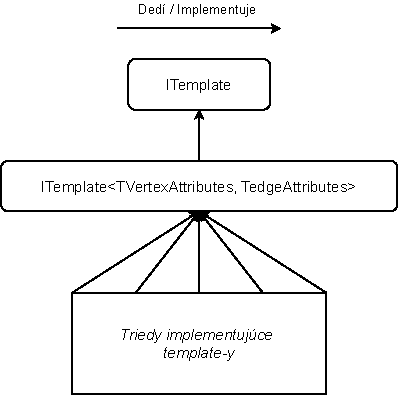
\includegraphics[]{img/templatey_architektura}
\caption{Diagram popisujúci objektovú štruktúru template-ov.} 
\label{obr05:templatey_architektura}
\end{figure}

\section{Mapy}

Táto oblasť sa stará o~vytváranie a~správu mapových objektov. Viac informácií o~koncepte Máp je možné nájsť v~Podsekcii~\ref{mapy}.

Hlavným uzlom pre~komunikáciu z~Model view vrstvy je singleton trieda \texttt{TemplateManager}. Tá ponúka kolekciu mapových formátov, ktorá obsahuje zástupcov všetkých mapových typov, ktoré~je možné v~aplikácii využiť. Každý zástupca zastupuje jeden typ mapy, jeden formát. Popri tom ponúka metódy pre~vytváranie mapových inštancií a~metódy pre~identifikáciu mapových formátov. 

V~následujúcich odsekoch popíšeme objektovú štruktúru máp a~ich~zástupcov. Grafické znázornenie tejto architektúry je možné nahliadnuť v~Diagrame~\ref{obr06:mapy_architektura}.   

\bigskip

Mapy sú reprezentované pomocou tried, ktoré~implementujú rozhranie \textbf{\texttt{IMap}}. Toto rozhranie nedefinuje žiadnu zaujímavú funkcionalitu. Obsahuje pár vlastností využívaných mimo vrstvy Model pre~identifikáciu mapy.

Triedy máp následne môžu implementovať niektoré z~ďalších definovaných rozhraní, ktoré~pridávajú svoje kontrakty. Tieto kontrakty sú zamerané na~geografické lokalizovanie a~rozlohu máp. Sú využívané predovšetkým pri~získavaní dodatočných výškových dát zodpovedajúcich konkrétnej mape. Ak si je mapový typ vedomý toho, že~na~vytvorenie jeho mapovej reprezentácie bude potrebná výpomoc výškových dát, mal by implementovať aspoň jeden z~interface-ov, ktorý~definuje informácie o~geo-lokalite a~rozlohe mapy.

Ako už bolo naznačené, pri~mapách je potrebné, aby~v~aplikácii niekto zastupoval ich formáty. K~tomuto slúžia triedy implementujúce trojicu rozhraní:
\begin{itemize}
    \item \textbf{\texttt{IMapFormat<out TMap>}} - Je určený pre~komunikáciu mimo vrstvy Model. Definuje vlastnosti, ktoré~sú potrebné pri~práci s~mapovým zástupcom vo~vonkajšom prostredí a~metódu na~vytváranie mapy zastupovaného typu. Tento interface by nemal byť priamo implementovaný.
    \item \textbf{\texttt{IMapIdentifier<in TMap>}} - Slúži na~identifikáciu zodpovedajúceho mapového formátu pre~konkrétny typ mapy. Vďaka kontravariantnej povahe jeho typového parametru bude táto identifikácia fungovať správne aj~pre~potomkov typu \texttt{TMap}. Tento interface by nemal byť priamo implementovaný.
    \item \textbf{\texttt{IMapRepresentative<TMap>}} - Zastupuje jeden konkrétny typ/formát mapy. Je potomkom predošlých dvoch interface-ov - spája ich funkcionality. Tento interface je určený k~tomu, aby~bol priamo implementovaný mapovými zástupcami.   
\end{itemize}

Na to, aby~bolo možné mapový typ využiť v~aplikácii, musí byť jeho zástupca zahrnutý v~príslušnej kolekcii v~triede \texttt{MapManager}. Z~tohto dôvodu je na~mieste, aby~boli títo zástupcovia implementovaní ako singleton triedy.

Mapy podporujú návrhový vzor \textit{Generic visitor pattern}. Ten je definovaný ako pre~rozhranie \texttt{IMap}, tak aj~pre~rozhranie \texttt{IGeoLocatedMap} (pridáva kontrakt o~geografickej lokalite mapy).

\begin{figure}[h]\centering
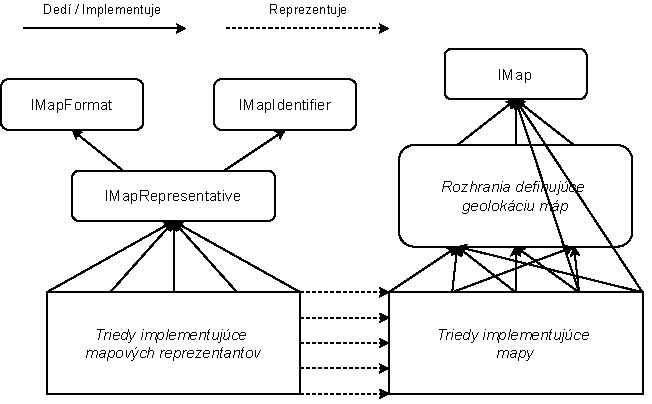
\includegraphics[]{img/mapy_architektura}
\caption{Diagram popisujúci objektovú štruktúru máp a ich zástupcov.} 
\label{obr06:mapy_architektura}
\end{figure}

\section{Mapové reprezentácie}

Ďalšia z~oblastí sa stará o~vytváranie a~spravovanie mapových reprezentácii, resp. grafov. Čo do~obsahu aj~komplexnosti sa jedná o~jednu z~najväčších oblastí. Viac informácií o~koncepte mapových reprezentácií je možné nájsť v~Podsekcii~\ref{mapove_reprezentacie}.

Hlavným uzlom pre~prácu s~touto oblasťou z~vonkajšieho prostredia je singleton trieda \texttt{MapRepreManager}. Ten ponúka kolekciu obsahujúcu zástupcov všetkých typov mapových reprezentácií, ktoré~je možné v~aplikácii využiť. Popri tom obsahuje metódy určené na~
\begin{itemize}
    \item vytváranie mapových reprezentácií,
    \item identifikáciu reprezentácií vytvoriteľných pre~konkrétnu kombináciu typov template-u a~mapy,
    \item detekciu potreby výškových dát pri~konštrukcii mapovej reprezentácie.
\end{itemize}

V~nasledujúcich odsekoch popíšeme objektovú štruktúru mapových reprezentácií/grafov, ich implementácií a~zástupcov. Pre~jednoduchšie porozumenie je možné v~Diagrame~\ref{obr07:mapove_reprezentacie_architektura} nahliadnuť grafické znázornenie tejto architektúry. 

\bigskip

Štruktúra dát, ktoré~súvisia s~mapovými reprezentáciami odzrkadľuje dvojakosť významov mapovej reprezentácie a~grafu ako bolo popísané v~Podsekcii~\ref{mapove_reprezentacie}. Každému typu mapovej reprezentácie je prisúdený konkrétny typ grafu.

Mapové reprezentácie/grafy sú v~aplikácii reprezentované triedami, ktoré~implementujú rozhranie \textbf{\texttt{IGraph<TVertex, TEdge>}}. Toto rozhranie reprezentuje myšlienku grafu, ktorý~zastupuje konkrétnu mapovú reprezentáciu. Jeho typové parametre definujú typy jeho vrcholov a~hrán. Obsahuje kontrakty, ktoré~musia grafy všetkých typov napĺňať. Aktuálne je to len jedna metóda vracajúca graf do~jeho základného stavu.

\texttt{IGraph<TVertexAttributes, TEdgeAttributes>} má za~predchodcu rozhranie \textbf{\texttt{IMapRepre}} reprezentujúce myšlienku samotnej mapovej reprezentácie. Cez toto rozhranie sú mapové reprezentácie/grafy distribuované vonkajšiemu svetu. K~tomuto účelu rozhranie definuje vlastnosti využívané mimo vrstvy Model. Grafová podstata mapových reprezentácií je tým vonkajšiemu svetu ukrytá a~len špecifické oblasti Model vrstvy ju znova odhaľujú a~využívajú.

Každá mapová reprezentácia/graf má množinu svojich implementácií. Implementácie sú tvorené pre~konkrétne kombinácie template-ov a~mapových formátov. Konkrétny typ mapovej reprezentácie môže byť vytvorený len pre~takú kombináciu template-u a~mapového formátu, pre~ktorý je vytvorená príslušná implementácia.

V~aplikácii sú naďalej prítomné ďalšie rozhrania, ktoré~môžu (a mali by v~čo najväčšom rozsahu) jednotlivé grafy implementovať. Tieto rozhrania definujú kontrakty týkajúce sa vlastností a~funkcií generovaných grafov.

\bigskip

Na to aby~mohla byť mapová reprezentácia, graf či~implementácia v~aplikácii použitá, musí pre~ne existovať vhodný zástupca. Tento zástupca je následne poskytnutý na~patričnom mieste.
\begin{itemize}
    \item Zástupcovia typov mapových reprezentácií sú v aplikácii reprezentovaní triedami, ktoré~implementujú rozhranie \textbf{\texttt{IMapRepreRepresentative<out TMapRepre>}}. Tieto triedy sú určené (podobne ako typy mapových reprezentácií) pre~komunikáciu mimo vrstvy Model. Definujú vlastnosti, ktoré~sú využívané vonkajším svetom pre~získanie informácií o~zastupovanej mapovej reprezentácii. 
    
    Nakoľko typ mapovej reprezentácia je vždy asociovaný s~nejakým typom grafu, zástupca typu mapovej reprezentácia disponuje aj~referenciou na~zástupcu typu daného grafu. Tento zástupca sa následne využíva v~procese vytvárania mapovej reprezentácie/grafu. Taktiež špecifické oblasti vrstvy Model ho môžu využiť k~otestovaniu vlastností zastupovaného grafu.

    Taktiež toto rozhranie definuje metódy pre~vytváranie zastupovaného typu mapovej reprezentácie. 

    Na~to, aby~bolo možné typ mapovej reprezentácie/grafu využiť v~aplikácii, musí byť jeho zástupca zahrnutý v~príslušnej kolekcii manažéra mapových reprezentácií.

    \item Zástupcovia grafových typov sú reprezentovaní triedami, ktoré~implementujú rozhranie \textbf{\texttt{IGraphRepresentative <out TGraph, TVertex, TEdge>}}. Typové parametre definujú typ zastupovaného grafu a~typy vrcholov a hrán, z ktorých je graf tvorený. Tento interface nedefinuje žiadny kontrakt pre~grafových zástupcov. Implementuje iba metódy, ktoré~sú využívané v~procese vytvárania mapovej reprezentácie/grafu. Je využívaný špecifickými oblasťami vrstvy Model k~otestovaniu vlastností zastupovaného grafu.

    Zástupcovia grafových typov si taktiež udržujú indikátorovú kolekciu zástupcov všetkých implementácií grafového typu. Táto kolekcia sa následne využíva pri~identifikácii použiteľných kombinácií template-ov a~mapových formátov a~pri samotnom vytváraní mapových reprezentácií/grafov.

    Každý zástupca grafu je asociovaný s~konkrétnym zástupcom mapovej reprezentácie. Ten si na~jeho inštanciu drží referenciu a~využíva ho v~procese vytvárania mapovej reprezentácie/grafu.

    \item Ku~reprezentácii zástupcov jednotlivých implementácií slúžia triedy, ktoré~dedia od abstraktnej triedy \textbf{\texttt{ElevDataIndepImplementationRep}} alebo~od abstraktnej triedy \textbf{\texttt{ElevDataDepImplementationRep}}. Tieto rozhrania disponujú dvojitou funkcionalitou:
    \begin{itemize}
        \item Obsahujú vlastnosti indikujúce template a~mapový formát, na~základe ktorých je implementácia mapovej reprezentácie/grafu agregovaná. Tieto vlastnosti sú naplnením kontraktu definovaného ich predchodcom \textbf{\texttt{IImplementationIndicator}}.
        \item Je schopná skonštruovať (alebo~nechať skonštruovať) zastúpenú implementáciu mapovej reprezentácie. Tieto triedy sa líšia predovšetkým v~potrebe dodatočných výškových dát v~procese tvorby danej implementácie. Schopnosť skonštruovať danú implementáciu je naplnením kontraktu jedného z~rozhraní \textbf{\texttt{IImplementationElevDataIndepConstr}}, respektíve \textbf{\texttt{IImplementationElevDataDepConstr}}. 
    \end{itemize}
    Taktiež disponujú množinou typových parametrov, z~ktorých každý má svoj špecifický význam:
    \begin{itemize}
        \item \texttt{TTemplate} - definuje typ template-u, pre~ktorý je zastupovaná implementácia vytvorená,
        \item \texttt{TGraph} - definuje typ mapovej reprezentácie/grafu, pre~ktorý je zastupovaná implementácia vytvorená,
        \item \texttt{TVertex, TEdge} - definujú typy vrcholov a hrán z ktorých sa skladá implementácia grafu,
        \item \texttt{TVertexAttributes, TEdgeAttributes} - definujú typy atribútov použitých v~implementovanom grafe,
        \item \texttt{TMap, TUsableSubMap} - tieto parametre sú jemne zavádzajúce. Prvý z~nich hovorí o~tom, aký typ mapy je navonok indikovaný pomocou vlastnosti mapového formátu. Druhý hovorí o~tom, ktorý~typ potomok typu \texttt{TMap} je v~skutočnosti potrebný na~vytvorenie mapovej reprezentácie. Malo by byť zaručené okolitým prostredím, že~pokiaľ je nejaká mapa správneho formátu, tak je určite možné ju použiť pre~vytvorenie mapovej reprezentácie. 
    \end{itemize}
    
    Zástupcovia jednotlivých implementácií mapovej reprezentácie sú zahrnutí v~kolekcii zástupcu tejto mapovej reprezentácie.

\end{itemize}

Bolo by vhodné, aby~všetci spomenutí zástupcovia boli implementovaní ako singleton triedy. Od každého z~nich je totiž za~celú dobu behu programu potrebné vytvoriť iba jedinú inštanciu, ktorá je poskytovaná zvyšku aplikácie na~patričnom mieste.

Poslednou súčasťou oblasti mapových reprezentácií sú triedy, ktoré~reprezentujú vrcholy a~hrany používané v~grafoch. Jednotlivé typy sa potom líšia dodávanými vlastnosťami.   

\begin{figure}[p]\centering
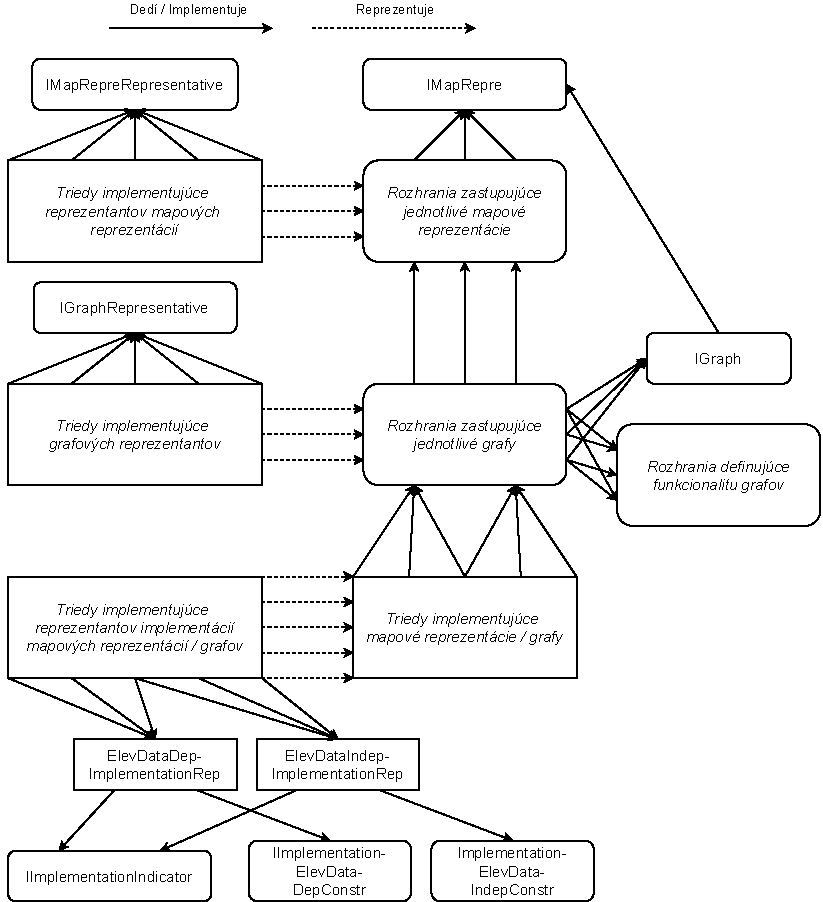
\includegraphics[]{img/mapove_reprezentacie_architektura}
\caption{Diagram popisujúci objektovú štruktúru mapových reprezentácií/grafov, ich implementácií a~zástupcov.} 
\label{obr07:mapove_reprezentacie_architektura}
\end{figure}

\pagebreak

\section{Užívateľské modely}

V~tejto oblasti sú vytvárané a~spravované užívateľské modely. Viac informácií o~koncepte užívateľských modelov je možné nájsť v~Podsekcii~\ref{uzivatelske_modely}.

Hlavným komunikačným uzlom s~touto oblasťou pre~Model view vrstvu je singleton trieda \texttt{UserModelManager}. Ten ponúka kolekciu všetkých typov užívateľských modelov, ktoré~je možné v~aplikácii využiť. Mimo to implementuje metódy pre:
\begin{itemize}
    \item Serializáciu a~deserializáciu užívateľských modelov do/z súborov,
    \item Vytváranie nových inštancií užívateľských modelov,
    \item Všeobecnú identifikáciu typov užívateľských modelov na~základe rôznych typov argumentov.
\end{itemize}

V~následujúcich odsekoch popíšeme objektovú štruktúru užívateľských modelov a~ich~zástupcov. Grafické znázornenie tejto architektúry je dostupné k nahliadnutiu v~Diagrame~\ref{obr08:uzivatelske_modely_architektura}.   

\bigskip

Užívateľské modely sú v~aplikácii reprezentované triedami, ktoré~implementujú rozhranie \textbf{\texttt{IUserModel<out TTemplate>}}.  Prostredníctvom tohto rozhrania sú užívateľské modely využívané mimo vrstvy Model. Z~tohto dôvodu definuje informatívne vlastnosti, ktoré~sú potrebné prevažne vo~vonkajšom svete. Popri tom definuje ešte aj~kontrakty zaručujúce schopnosť serializácie užívateľského modelu. Každý užívateľský model je viazaný na~konkrétny template, typu \texttt{TTemplate}. K~tomu si každý užívateľský model nesie aj~referenciu na~inštanciu daného template-u.

Na to aby~bol užívateľský model použiteľný vo~vyhľadávacích algoritmoch, nestačí aby~implementoval predchádzajúce základné rozhranie. Je potrebné aby~implementoval následnícke rozhranie \textbf{\texttt{IComputingUserModel<out TTemplate, in TVertexAttributes, in TEdgeAttributes>}}. Tento interface sám o~sebe nedefinuje žiadny kontrakt. Až jeho následníci definujú výpočtovú funkcionalitu, ktorú implementujúci užívateľský model vie ponúknuť napríklad vyhľadávaciemu algoritmu. 

Jedným z~týchto následníkov je interface \textbf{\texttt{IWeightComputingUserModel<out TTemplate, in TVertexAttributes, in TEdgeAttributes>}}. Toto rozhranie zaisťuje schopnosť užívateľského modelu, na~základe dodaných vrcholových a~hranových atribútov, vypočítať váhu zodpovedajúcej hrany. Túto funkcionalitu by mali spĺňať všetky užívateľské modely, nakoľko veľká časť vyhľadávacích algoritmov potrebuje poznať váhu jednotlivých hrán pre~správny výber postupu.

Oproti výpočtovým rozhraniam existuje v~tejto oblasti aj~špecifické rozhranie \textbf{\texttt{ISettableUserModel}}. Toto rozhranie musia implementovať všetky typy užívateľských modelov, ktoré~sú určené na~to, aby~v~nich užívateľ mohol konfigurovať nastaviteľné hodnoty (tzv.\textit{Adjustables}) vzhľadom na~svoje preferencie. Kontrakt ktorý~definuje zaručuje dodanie kolekcie týchto nastaviteľných hodnôt, aby~mohli byť dodané užívateľovi a~ten s~nimi mohol pracovať. Mechanizmus vytvárania a~nastavovania užívateľských modelov zatiaľ v~aplikácii nie je implementovaný, a~teda toto rozhranie aktuálne čaká na~svoje využitie.  

\bigskip

V~aplikácii je potrebné, aby~existencia jednotlivých typov užívateľských modelov bola nejakým spôsobom zastúpená. Týmito zástupcami sú triedy implementujúce následujúcu trojicu rozhraní:
\begin{itemize}
    \item \textbf{\texttt{IUserModelType<out TUserModel, out TTemplate>}} - Je určený pre~komunikáciu mimo vrstvy Model. Definuje vlastnosti, ktoré~sú potrebné pri~práci so~zástupcom užívateľského modelu vo~vonkajšom prostredí. 
    
    Taktiež obsahuje referenciu na~template, na~ktorý je zastupovaný užívateľský model viazaný a~definuje metódy slúžiace na~deserializáciu a~vytváranie nových užívateľských modelov. Implementácie deserializácie zástupcu a~serializácie zastupovaného užívateľského modelu sa musia zhodovať. 
    
    Tento interface by nikdy nemal byť priamo implementovaný.
    \item \textbf{\texttt{IUserModelTemplateBond<in TTemplate>}} - Reprezentuje väzbu užívateľského modelu a~template-u. Vďaka kontravariantnej povahe jeho template-ového typového parametru bude táto identifikácia fungovať správne aj~pre~prípadných potomkov typu \texttt{TTemplate}. Tento interface by nikdy nemal byť priamo implementovaný.
    \item \textbf{\texttt{IUserModelIdentifier<in TUserModel>}} - Identifikuje individuálny užívateľský model alebo~jeho potomkov. Vďaka kontravariantnej povahe jeho typového parametru bude táto identifikácia fungovať správne aj~pre~potomkov typu \texttt{TUserModel}. Tento interface by nikdy nemal byť priamo implementovaný.
    \item \textbf{\texttt{UserModelRepresentative<TUserModel,TTemplate,TConfiguration>}} - Zastupuje jeden konkrétny typ užívateľského modelu viazaného na~jeden konkrétny typ template-u. Je potomkom predošlých troch interface-ov - spája ich funkcionality. Táto trieda je určený k~tomu, aby~z~nej priamo dedili zástupcovia užívateľských modelov.   
\end{itemize}

Na to, aby~bolo možné typ užívateľského modelu využiť v~aplikácii, musí byť jeho zástupca zahrnutý v~príslušnej kolekcii triedy \texttt{UserModelManager}. Z~tohto dôvodu je na~mieste, aby~títo zástupcovia boli implementovaný ako singleton-y.

\begin{figure}[h]\centering
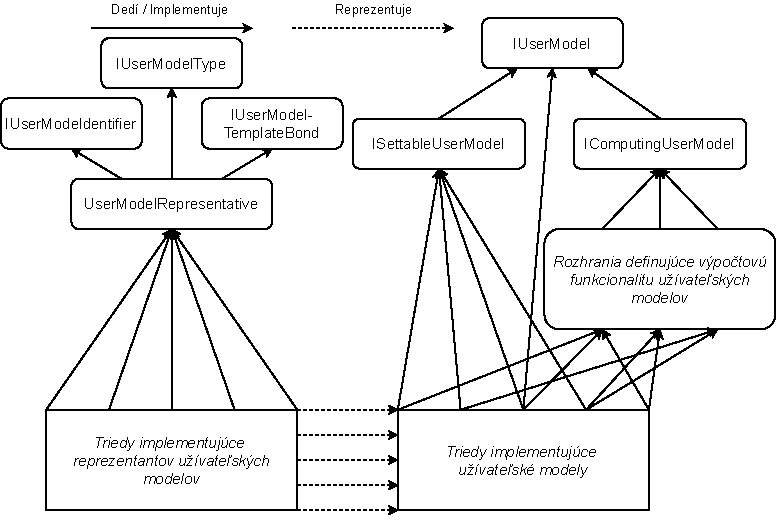
\includegraphics[]{img/uzivatelske_modely_architektura}
\caption{Diagram popisujúci objektovú štruktúru užívateľských modelov a~ich~zástupcov.} 
\label{obr08:uzivatelske_modely_architektura}
\end{figure}

\section{Vyhľadávacie algoritmy}

Táto oblasť zahŕňa mechanizmy spravujúce algoritmy pre~vyhľadávanie ciest v~mapových reprezentáciách. Viac informácií o~vyhľadávacích algoritmoch samotných je možné nájsť v~Podsekcii~\ref{vyhladavacie_algoritmy}. 

Hlavným komunikačným uzlom s~touto oblasťou pre~Model view vrstvu je singleton trieda \texttt{SearchingAlgorithmMan}. Táto trieda zverejňuje v~kolekcii všetky použiteľné vyhľadávacie algoritmy aplikácie. Popri tom obsahuje metódy zabezpečujúce: 
\begin{itemize}
    \item spúšťanie procesu vyhľadávania cesty na~základe dodaného užívateľského modelu a~mapovej reprezentácie
    \item dodávanie \textit{executor}-u vyhľadávacieho algoritmu
    \item identifikáciu vyhľadávacích algoritmov spustiteľných pre~konkrétne kombinácie mapových reprezentácií a~užívateľských modelov 
\end{itemize}

V~následujúcich odsekoch popíšeme objektovú štruktúru vyhľadávacích algoritmov a~ich~implementácií. Jednoduché grafické znázornenie tejto architektúry je dostupné k nahliadnutiu v~Diagrame~\ref{obr09:vyhladavacie_algoritmy_architektura}.   

\bigskip

Vyhľadávacie algoritmy sú v~aplikácii reprezentované pomocou tried, ktoré~implementujú rozhranie \textbf{\texttt{ISearchingAlgorithm}}. Každý algoritmus môže byť implementovaný niekoľkými spôsobmi. Rozhranie preto definuje kolekciu, v~ktorej by mali byť všetky použiteľné implementácie daného algoritmu zverejnené. Ďalej definuje a~zároveň implementuje metódy, ktoré~slúžia na:
\begin{itemize}
    \item testovanie, či~zástupcovia typov mapovej reprezentácie a~užívateľského modelu zastupujú použiteľnú kombináciu pre~daný algoritmus. Teda či~existuje implementácia algoritmu, pre~ktorú sú vlastnosti zastupovaných typov dostatočné na~použitie, 
    \item samotné spúšťanie vyhľadávacieho procesu. K~tomuto účelu sa vyberie pre~vstupné argumenty vhodná implementácia algoritmu,
    \item možnosť získania \textit{executor}-u daného algoritmu. Executor sa vytvorí na~základe vhodnej implementácie algoritmu.
\end{itemize}
Inštancia každého použiteľného vyhľadávacieho algoritmu musí byť obsiahnutá v~kolekcii vyhľadávacích algoritmov v~príslušnom manažérovi. Inak nebude aplikácia daný vyhľadávací algoritmus registrovať. 

Implementácie vyhľadávacích algoritmov sú reprezentované triedami, ktoré~implementujú rozhranie \textbf{\texttt{ISearchingAlgorithmImplementation}}. Toto rozhranie definuje myšlienky funkcionalít podobné tým z~rozhrania \texttt{ISearchingAlgorithm}: testovanie typov vstupných mapových reprezentácií a~užívateľských modelov, spúšťanie vyhľadávacieho procesu a~vytváranie svojich executor-ov. V~tomto prípade však nie je táto funkcionalita implementovaná rozhraním a~je potrebné aby~ju implementácie algoritmov doplnili sami. Na~to aby~implementácia algoritmu mohla byť použitá, musí byť obsiahnutá v~kolekcii implementácií zodpovedajúceho vyhľadávacieho algoritmu. 

Výsledkom vyhľadávania je inštancia triedy, ktorá implementuje rozhranie \textbf{\texttt{IPath<out TVertexAttributes, out TEdgeAttributes>}}. Toto rozhranie reprezentuje nájdenú cestu algoritmom pričom môže v~sebe niesť atribúty typov \texttt{TVertexAttributes} a~\texttt{TEdgeAttributes}. Neskôr v~Model view vrstve je z~tejto cesty vytvorený report, ktorý~je následne vyššími vrstvami spracovaný a~predvedený užívateľovi. Pre~komunikáciu mimo Model vrstvy sa využíva jeho predchodca \texttt{IPath}. Toto rozhranie by nemalo byť nikdy priamo implementované. 

Vyhľadávacie algoritmy taktiež môžu počas svojho behu podávať report-y o~stave vyhľadávania prostredníctvom objektov tried, ktoré~implementujú rozhranie \textbf{\texttt{ISearchingState<out TVertexAttributes, out TEdgeAttributes>}}. Algoritmus nechá z~týchto stavov agregovať report a~podá ho k~následnému spracovaniu a~predvedeniu užívateľovi.

Obidve vyššie spomenuté rozhrania taktiež podporujú návrhový vzor \textit{generic visitor pattern}. 

Pokiaľ je po~algoritme požadované vytvorenie jeho executor-u, algoritmus zavolá vhodnú svoju implementáciu nech executor vytvorí. Tá ho inicializuje pomocou dodanej mapovej reprezentácie, užívateľského modelu a~pridá delegáta na~svoju špecifickú metódu zabezpečujúcu beh algoritmu pre~executor.

Všetky triedy reprezentujúce vyhľadávacie algoritmy a~ich implementácie by mali byť implementované ako singleton triedy. Ich inštancie budú totiž vytvorené v~aplikácii len jeden krát.


\begin{figure}[h]\centering
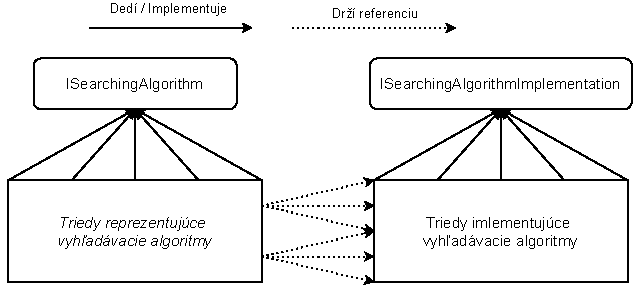
\includegraphics[]{img/vyhladavacie_algoritmy_architektura}
\caption{Diagram popisujúci objektovú štruktúru vyhľadávacích algoritmov a~ich~implementácií.} 
\label{obr09:vyhladavacie_algoritmy_architektura}
\end{figure}

\pagebreak

\section{Výškové dáta}

Oblasť pre~správu a~manipuláciu s~výškovými dátami. Viac informácií o~funkcii výškových dát v~aplikácii je možné nájsť v~Podsekcii~\ref{vyskove_data}. 

Hlavným komunikačným uzlom s~touto oblasťou z~vrstvy Model view je singleton trieda \texttt{ElevDataManager}. Tá ponúka kolekciu všetkých použiteľných zdrojov výškových dát v~aplikácii. Popri tom doručuje metódy pre~manipuláciu s~výškovými dátami (sťahovanie a~odstraňovanie) a~taktiež metódy, ktoré~testujú prítomnosť a~vracajú prítomné výškové dáta zodpovedajúce rozlohe konkrétnej mapy.

V~následujúcich odsekoch popíšeme objektovú štruktúru výškových dát, ich zdrojov, distribúcií a~regiónov. Pre lepšie porozumenie je v~Diagrame~\ref{obr10:vyskove_data_architektura} dostupný náhľad  grafického znázornenia architektúry týchto dátových štruktúr.   

\bigskip

Výškové dáta sú v~aplikácii reprezentované triedami, ktoré~implementujú rozhranie \textbf{\texttt{IElevData}}. Toto jednoduché rozhranie definuje metódy, ktoré~dokážu k~zadanej geografickej polohe vrátiť jej nadmorskú výšku. Inštancie týchto tried su na~mieru vytvárané tak, aby~dokázali dodať výškové dáta primerané polohe a~rozlohe konkrétnej mapy. 

Výškové dáta sú dodávané jednotlivými zdrojmi. Tie sú v~aplikácii reprezentované triedami, ktoré~implementujú rozhranie \textbf{\texttt{IElevDataSource}}. Zdroje výškových dát sú zložené z~viacerých distribúcií, ktoré~následne už dodávajú potrebnú funkcionalitu pre~prácu s~nimi spravovanými, výškovými dátami. Preto rozhranie \texttt{IElevDataSource} definuje kolekciu, v~ktorej by mali byť uložené všetky distribúcie daného zdroja na~to, aby~mohli byť v~aplikácii použité. Popri tom definuje ďalších pár vlastností, ktoré~sú využívané mimo vrstvy Model (napr. meno daného zdroja).

Jednotlivé distribúcie výškových dát sú v~aplikácii reprezentované triedami, ktoré~implementujú rozhranie \textbf{\texttt{IElevDataDistribution}}. Každá z~týchto tried je zodpovedná za~prácu s~konkrétnou distribúciou výškových dát. Zabezpečujú sťahovanie, odstraňovanie a~informovanie o~ich prítomnosti. Je ponechané na~zodpovednosti implementácií, akým spôsobom budú dáta ukladané, načítané do~pamäte a~spracovávané do~inštancií implementácií rozhrania \texttt{IElevData}.

Rozhranie \texttt{IElevDataDistribution} by nemalo byť implementované priamo. Namiesto toho by mali byť implementované rozširujúce rozhrania \textbf{\texttt{ICredentials-} \texttt{NotRequiringElevDataDistribution}} a~\textbf{\texttt{ ICredentialsRequiringElevData- } \texttt{Distribution}},  ktoré~pridávajú samotnú metódu umožňujúcu sťahovanie výškových dát. Tieto metódy, resp. rozhrania, sa líšia v~potrebe autorizácie pri~získavaní výškových dát zo~vzdialených zdrojov.  

Manipulovanie s~výškovými dátami prebieha po~takzvaných \textit{regiónoch}. Každá distribúcia si tvar a~veľkosť svojich regiónov určuje sama. Následne tieto regióny sprostredkováva v~kolekcii \texttt{AllTopRegions}, ktorá je definovaná rozhraním \texttt{IElevDataDistribution}.

Regióny sú reprezentované triedami, ktoré~dedia od abstraktnej triedy \textbf{\texttt{Region}} a~jej potomkov \textbf{\texttt{TopRegion}} a~\textbf{\texttt{SubRegion}}. Región ako taký definuje svoje meno, svoj tvar za~pomoci reťazca geografických súradníc a~množinu svojich pod-regiónov. Taktiež definuje identifikátor svojej prítomnosti. Teda toho, čí sú jemu zodpovedajúce výškové dáta stiahnuté v~počítači a~pripravené na~použitie alebo~nie.

Tento indikátor by mal byť aktualizovaný vždy keď sa prítomnosť dát regiónu zmení. Dôležité však je, že~táto informácia by mala byť zachovaná naprieč behmi aplikácie. Teda ak sú v~jednom behu aplikácie stiahnuté výškové dáta pre~konkrétny región, v~následujúcom behu by mal región indikovať, že~sú jemu prislúchajúce dáta stále k~dispozícii.

Regióny sú naďalej delené na~\textit{vrcholové regióny} a~\textit{pod-regióny}. Pod-regióny sú vždy viazané na~nejaký vyšší región a~reprezentujú nejakú jeho časť. Vrcholový región potom jednoducho nie je nikoho pod-regiónom. Spomínaná kolekcia \texttt{AllTopRegions} obsahuje práve vrcholové regióny definované danou distribúciou.    


\begin{figure}[h]\centering
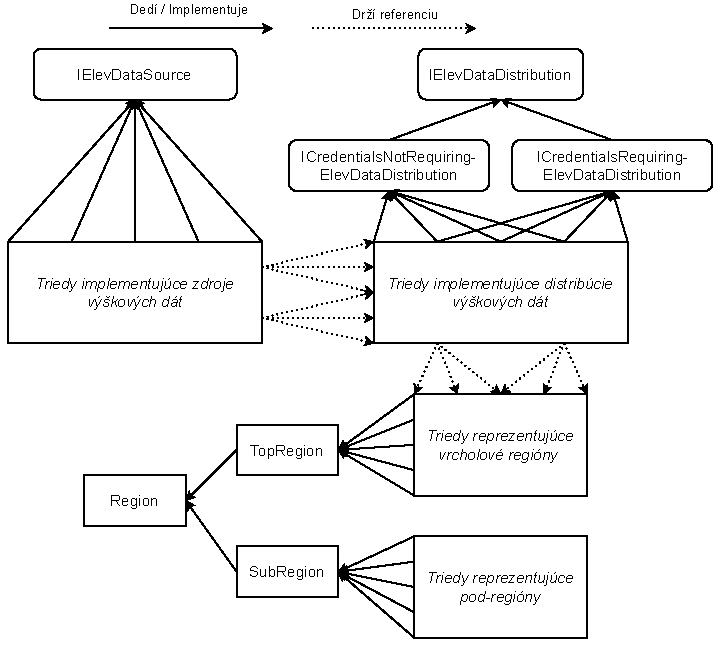
\includegraphics[]{img/vyskove_data_architektura}
\caption{Diagram popisujúci objektovú štruktúru zdrojov, distribúcií a~regiónov výškových dát.} 
\label{obr10:vyskove_data_architektura}
\end{figure}

\pagebreak

\section{Grafika}

Táto oblasť sa zaoberá problematikou vytvárania objektov, z~ktorých sa skladajú grafické reprezentácie rôznych dátových štruktúr. Agregácia grafických objektov sa vykonáva špecifickým asynchrónnym postupom. Vytvorené grafické objekty sa plnia do~tzv \textit{kolektoru}. Tým pádom je možné vytvorené objekty paralelne spracovávať a~zobrazovať ihneď po~ich vytvorení. 

Aplikácia obsahuje hneď dva hlavné uzly pre~komunikáciu s~touto oblasťou:
\begin{itemize}
    \item \texttt{GraphicsManager} je hlavným uzlom pre~komunikáciu prichádzajúcu z~Model view vrstvy. Zabezpečuje agregáciu grafických objektov pre~rôzne dátové štruktúry aplikácie ako sú napríklad mapy.
    \item \texttt{GraphicsSubManager} slúži k~rovnakému účelu ako \texttt{GraphicsManager}, avšak pre~komunikáciu priamo z~vrstvy Model. Reprezentuje prívetivejší spôsob komunikácie so~zachovaním typových informácií. Dátové štruktúry, pre~ktoré zabezpečuje táto trieda agregáciu grafiky, sú napríklad nájdené cesty a~stavy vyhľadávacích algoritmov. 
\end{itemize}
Obidve tieto triedy sa riadia návrhovým vzorom singleton.

\bigskip

Grafické objekty sú v~aplikácii reprezentované triedami, ktoré~implementujú rozhranie \textbf{\texttt{IGraphicObject}}.Toto rozhranie neimplementuje takmer žiadnu funkcionalitu okre podpory návrhového vzoru \textit{Generic visitor pattern}.

Aby bolo možné grafiku dodanej mapy, cesty či~stavu extrahovať, musí pre~ňu existovať trieda implementujúca rozhranie \textbf{\texttt{IGraphicsAggregator}}, teda presnejšie jedného z~jeho špecializovaných potomkov. Títo \textit{agregátori} následne dostanú objekt na~spracovanie a~kolektor, do~ktorého sa majú naklásť vytvorené grafické objekty.

V~prípade ciest a~stavov vyhľadávacieho algoritmu dostane agregátor aj~užívateľský model, ktorý~môže využiť na~výpočet niektorých hodnôt z~vrcholových a~hranových atribútov uložených v~dodaných cestách/stavoch. Je však potrebné zdôrazniť, že~užívateľský model možno nebude schopný tieto služby doručiť. V~takom prípad sa musí agregátor zaobísť bez nich. Je možnosť, aby~tieto vlastnosti vynucoval napríklad vyhľadávací algoritmus, ktorý~pozná potreby pre~extrahovanie grafiky ním používaného typu cesty či~stavu vyhľadávania.

Bolo by namieste, keby každý užívateľský model dokázal z~atribútov vyťažiť aspoň pozície vrcholov mapovej reprezentácie, aby~bolo možné nakresliť aspoň základnú reprezentáciu nájdenej cesty či~stavu. 

\bigskip

Nakoniec sú v~tejto oblasti definované dve rozhrania ktoré~slúžia pre~reprezentáciu grafického zdroja. \textbf{\texttt{IGraphicsSource}} definuje jedinú vlastnosť a~to zdrojovú kolekciu grafických objektov. Táto zdrojová kolekcia je typu \texttt{SourceList} patriaceho do~framework-u \textit{Reactive UI}. vo~vyšších vrstvách MVVM(MV) architektúry je následne možné tento zdrojový zoznam sledovať a~reagovať na~jeho aktualizácie. 

Špecializácia predošlého rozhrania \textbf{\texttt{IGroundGraphicsSource}} dodáva ešte nutnosť, aby~daný grafický zdroj definoval aj~svoju rozlohu. Triedy implementujúce toto rozhranie sú často využívané ako akési základné grafiky, ktorých rozlohe sa ostatné grafické zdroje prispôsobujú.

Implementácie týchto rozhraní sú väčšinou vytvárané mimo vrstvy Model. Sú na~mieru vytvorené pre~konkrétnu aplikačnú logiku. 

\section{Reportovanie}

Oblasti spravujúcej grafiku je architektúrou veľmi podobná oblasť vytvárajúca report-y na~základe rôznych typov dátových štruktúr. V~aktuálnej podobe aplikácie sú týmito štruktúrami cesty, nájdené vyhľadávacími algoritmami a~stavy vyhľadávacích algoritmov. Táto oblasť veľmi často využíva služby triedy \texttt{GraphicsSubManager} pre~získavanie grafiky, ktorá je pridaná do~obsahu report-ov.

Oblasť obsahuje opäť dva hlavné komunikačné uzly:
\begin{itemize}
    \item \texttt{ReportManager} je hlavným uzlom pre~komunikáciu prichádzajúcu z~Model view vrstvy. Aktuálne zabezpečuje vytváranie report-ov pre~nájdené cesty vyhľadávacím algoritmom.
    \item \texttt{ReportSubManager} slúži k~rovnakému účelu ako \texttt{ReportManager}, avšak pre~komunikáciu priamo z~vrstvy Model. Reprezentuje prívetivejší spôsob komunikácie so~zachovaním typovej informácie. Aktuálne zabezpečuje vytváranie report-ov pre~nájdené cesty a~stavy vyhľadávaní.
\end{itemize}
Obidve tieto triedy sa riadia návrhovým vzorom singleton.

\bigskip

Pre cesty a~stavy vyhľadávania sú reporty v~aplikácii reprezentované triedami, ktoré~implementujú rozhrania \textbf{\texttt{IPathReport}} a~\textbf{\texttt{ISearchingReport}}. Tieto rozhrania nedefinujú takmer žiadnu funkcionalitu, okrem podpory návrhového vzoru \textit{generic visitor pattern}.

Podobne ako v~oblasti spravujúcej grafiku, na~to, aby~pre~konkrétny typ dátovej štruktúry mohol byť report vytvorený, musí preňho existovať vhodná trieda implementujúca rozhranie \textbf{\texttt{IReportAggregator}}, resp. jedného z~jeho špecializovaných potomkov. Títo \textit{agregátori} následne dostanú dátovú štruktúru na~spracovanie a~v~niektorých prípadoch aj~užívateľský model, ktorý~môžu využiť na~výpočet hodnôt z~vrcholových a~hranových atribútov uložených v~dodaných dátach. Podobne však ako u grafických agregátorov, nie je zaručené, že~užívateľský model bude schopný požadované služby doručiť. 

\section{Parametre}

Posledná, jednoduchšia, ale~o~to dôležitejšia, oblasť je využívaná na~spravovanie a~ukladanie všemožných parametrov aplikácie. Hlavným uzlom pre~komunikáciu s~touto oblasťou je singleton trieda \texttt{ParamsManager}. V~tejto triede je možné uložiť od každého typu parametrov práve jednu inštanciu. Táto inštancia môže byť počas behu algoritmu rôzne upravovaná. Inštancie parametrov sú uložené v~slovníku pod kľúčom reprezentujúcom ich vlastný typ.  

Keď je zavolaná metóda \texttt{SaveAllParams}, tak sa trieda \texttt{ParamsManager} pokúsi všetky uložené parametre v~slovníku serializovať do~súborov pre~možnosť ich použitia v~budúcich behoch aplikácie.

Pri následnom behu aplikácie sú parametre deserializované zo~súborov tzv. \uv{lenivým} spôsobom. Keď je požiadané o~parametre typu, ktorý~v~slovníku nie je zastúpený, trieda sa pokúsi najprv zistiť, či~preňho neexistuje zodpovedajúca serializácia. Ak áno, deserializuje sa inštancia zodpovedajúcich parametrov, vloží sa do~slovníku a~vráti užívateľovi. Pokiaľ nie, poznačí sa do~slovníku neexistencia parametru daného typu a~navráti sa hodnota \texttt{null}.  

Serializácia a~deserializácia parametrov do~súborov, v~ktorých prežívajú beh aplikácie, prebieha za~pomoci singleton triedy \textbf{\texttt{DataSerializer}}. Táto trieda serializuje objekty do~súborov pomocou systémovej triedy \textit{\texttt{JsonSerializer}}. Súbory sú pomenované podľa typu daného serializovaného objektu. To znamená, že~v~jednu chvíli pre~každý dátový typ dokáže táto trieda serializovať jednu jedinú inštanciu. Pri~deserializácii, na~základe vstupného generického typového parametru nájde súbor so~zodpovedajúcim menom a~pokúsi sa ho deserializovať do~inštancie daného typu.


  

% %%% Fiktivní kapitola s ukázkami sazby

\chapter{Nápověda k~sazbě}

\section{Úprava práce}

Vlastní text práce je uspořádaný hierarchicky do kapitol a podkapitol,
každá kapitola začíná na nové straně. Text je zarovnán do bloku. Nový odstavec
se obvykle odděluje malou vertikální mezerou a odsazením prvního řádku. Grafická
úprava má být v~celém textu jednotná.

Práce se tiskne na bílý papír formátu A4. Okraje musí ponechat dost místa na vazbu:
doporučen je horní, dolní a pravý okraj $25\,\rm mm$, levý okraj $40\,\rm mm$.
Číslují se všechny strany kromě obálky a informačních stran na začátku práce;
první číslovaná strana bývá obvykle ta s~obsahem.

Písmo se doporučuje dvanáctibodové ($12\,\rm pt$) se standardní vzdáleností mezi řádky
(pokud píšete ve Wordu nebo podobném programu, odpovídá tomu řádkování $1,5$; v~\TeX{}u
není potřeba nic přepínat).

Primárně je doporučován jednostranný tisk (příliš tenkou práci lze obtížně svázat).
Delší práce je lepší tisknout oboustranně a přizpůsobit tomu velikosti okrajů:
$40\,\rm mm$ má vždy \emph{vnitřní} okraj. Rub titulního listu zůstává nepotištěný.

Zkratky použité v textu musí být vysvětleny vždy u prvního výskytu zkratky (v~závorce nebo
v poznámce pod čarou, jde-li o složitější vysvětlení pojmu či zkratky). Pokud je zkratek
více, připojuje se seznam použitých zkratek, včetně jejich vysvětlení a/nebo odkazů
na definici.

Delší převzatý text jiného autora je nutné vymezit uvozovkami nebo jinak vyznačit a řádně
citovat.

\section{Jednoduché příklady}

K~různým účelům se hodí různé typy písma.
Pro běžný text používáme vzpřímené patkové písmo.
Chceme-li nějaký pojem zvýraznit (třeba v~okamžiku definice), používáme obvykle
\textit{kurzívu} nebo \textbf{tučné písmo.}
Text matematických vět se obvykle tiskne pro zdůraznění \textsl{skloněným (slanted)} písmem;
není-li k~dispozici, může být zastoupeno \textit{kurzívou.}
Text, který je chápan doslova (například ukázky programů) píšeme \texttt{psacím strojem}.
Důležité je být ve volbě písma konzistentní napříč celou prací.

Čísla v~českém textu obvykle sázíme v~matematickém režimu s~desetinnou čárkou:
%%% Bez \usepackage{icomma}:
% $\pi \doteq 3{,}141\,592\,653\,589$.
%%% S \usepackage{icomma}:
$\pi \doteq 3,141\,592\,653\,589$.
V~matematických textech je často lepší používat desetinnou tečku
(pro lepší odlišení od čárky v~roli oddělovače).
Nestřídejte však obojí.
Numerické výsledky se uvádějí s~přiměřeným počtem desetinných míst.

Mezi číslo a jednotku patří úzká mezera: šířka stránky A4 činí $210\,\rm mm$, což si
pamatuje pouze $5\,\%$ autorů. Pokud ale údaj slouží jako přívlastek, mezeru vynecháváme:
$25\rm mm$ okraj, $95\%$ interval spolehlivosti.

Rozlišujeme různé druhy pomlček:
červeno-černý (krátká pomlčka),
strana 16--22 (střední),
$45-44$ (matematické minus),
a~toto je --- jak se asi dalo čekat --- vložená věta ohraničená dlouhými pomlčkami.

V~českém textu se používají \uv{české} uvozovky, nikoliv ``anglické''.

% V tomto odstavci se vlnka zviditelňuje
{
\def~{{\tt\char126}}
Na některých místech je potřeba zabránit lámání řádku (v~\TeX{}u značíme vlnovkou):
u~předložek (neslabičnych, nebo obecně jednopísmenných), vrchol~$v$, před $k$~kroky,
a~proto, \dots{} obecně kdekoliv, kde by při rozlomení čtenář \uv{ško\-brt\-nul}.
}

\section{Matematické vzorce a výrazy}

Proměnné sázíme kurzívou (to \TeX{} v~matematickém módu dělá sám, ale
nezapomínejte na to v~okolním textu a také si matematický mód zapněte).
Názvy funkcí sázíme vzpřímeně. Tedy například:
$\var(X) = \E X^2 - \bigl(\E X \bigr)^2$.

Zlomky uvnitř odstavce (třeba $\frac{5}{7}$ nebo $\frac{x+y}{2}$) mohou
být příliš stísněné, takže je lepší sázet jednoduché zlomky s~lomítkem:
$5/7$, $(x+y)/2$.

Není předepsáno, jakým písmem označovat jednotlivé druhy matematických objektů
(matice, vektory, atd.), ale značení pro tentýž druh objektu musí být v~celé
práci používáno stejně. Podobně používáte-li více různých typů závorek, je třeba
dělat to v~celé práci konzistentně.

Nechť
\[   % LaTeXová náhrada klasického TeXového $$
\mathbf{X} = \begin{pmatrix}
      \T{\bm x_1} \\
      \vdots \\
      \T{\bm x_n}
      \end{pmatrix}.
\]
Povšimněme si tečky za~maticí. Byť je matematický text vysázen
ve~specifickém prostředí, stále je gramaticky součástí věty a~tudíž je
zapotřebí neopomenout patřičná interpunkční znaménka. Obecně nechceme
sázet vzorce jeden za druhým a raději je propojíme textem.

Výrazy, na které chceme později odkazovat, je vhodné očíslovat:
\begin{equation}\label{eq01:Xmat}
\mathbf{X} = \begin{pmatrix}
      \T{\bm x_1} \\
      \vdots \\
      \T{\bm x_n}
      \end{pmatrix}.
\end{equation}
Výraz \eqref{eq01:Xmat} definuje matici $\mathbf{X}$. Pro lepší čitelnost
a~přehlednost textu je vhodné číslovat pouze ty výrazy, na které se
autor někde v~další části textu odkazuje. To jest, nečíslujte
automaticky všechny výrazy vysázené některým z~matematických
prostředí.

Zarovnání vzorců do několika sloupečků:
\begin{alignat*}{3}
S(t) &= \pr(T > t),    &\qquad t&>0       &\qquad&\text{ (zprava spojitá),}\\
F(t) &= \pr(T \leq t), &\qquad t&>0       &\qquad&\text{ (zprava spojitá).}
\end{alignat*}

Dva vzorce se spojovníkem:
\begin{equation}\label{eq01:FS}
\left.
\begin{aligned}
S(t) &= \pr(T > t) \\[1ex]
F(t) &= \pr(T \leq t)
\end{aligned}
\;	% zde pomůže ručně vynechat trochu místa
\right\}
\quad t>0 \qquad \text{(zprava spojité).}
\end{equation}

Dva centrované nečíslované vzorce:
\begin{gather*}
\bm Y = \mathbf{X}\bm\beta + \bm\varepsilon, \\[1ex]
\mathbf{X} = \begin{pmatrix} 1 & \T{\bm x_1} \\ \vdots & \vdots \\ 1 &
  \T{\bm x_n} \end{pmatrix}.
\end{gather*}
Dva centrované číslované vzorce:
\begin{gather}
\bm Y = \mathbf{X}\bm\beta + \bm\varepsilon, \label{eq02:Y}\\[1ex]
\mathbf{X} = \begin{pmatrix} 1 & \T{\bm x_1} \label{eq03:X}\\ \vdots & \vdots \\ 1 &
  \T{\bm x_n} \end{pmatrix}.
\end{gather}

Definice rozdělená na dva případy:
\[
P_{r-j}=
\begin{cases}
0, & \text{je-li $r-j$ liché},\\
r!\,(-1)^{(r-j)/2}, & \text{je-li $r-j$ sudé}.
\end{cases}
\]
Všimněte si použití interpunkce v této konstrukci. Čárky a tečky se
dávají na místa, kam podle jazykových pravidel patří.

\begin{align}
x& = y_1-y_2+y_3-y_5+y_8-\dots = && \text{z \eqref{eq02:Y}} \nonumber\\
& = y'\circ y^* = && \text{podle \eqref{eq03:X}} \nonumber\\
& = y(0) y' && \text {z Axiomu 1.}
\end{align}


Dva zarovnané vzorce nečíslované (povšimněte si větších závorek, aby se do nich
vešel vyšší vzorec):
\begin{align*}
L(\bm\theta) &= \prod_{i=1}^n f_i(y_i;\,\bm\theta), \\
\ell(\bm\theta) &= \log\bigl\{L(\bm\theta)\bigr\} =
\sum_{i=1}^n \log\bigl\{f_i(y_i;\,\bm\theta)\bigr\}.
\end{align*}
Dva zarovnané vzorce, první číslovaný:
\begin{align}
L(\bm\theta) &= \prod_{i=1}^n f_i(y_i;\,\bm\theta), \label{eq01:L} \\
\ell(\bm\theta) &= \log\bigl\{L(\bm\theta)\bigr\} =
\sum_{i=1}^n \log\bigl\{f_i(y_i;\,\bm\theta)\bigr\}. \nonumber
\end{align}

Vzorec na dva řádky, první řádek zarovnaný vlevo, druhý vpravo, nečíslovaný:
\begin{multline*}
\ell(\mu,\,\sigma^2) = \log\bigl\{L(\mu,\,\sigma^2)\bigr\} =
\sum_{i=1}^n \log\bigl\{f_i(y_i;\,\mu,\,\sigma^2)\bigr\}= \\
  = -\,\frac{n}{2}\,\log(2\pi\sigma^2) \,-\,
\frac{1}{2\sigma^2}\sum_{i=1}^n\,(y_i - \mu)^2.
\end{multline*}

Vzorec na dva řádky, zarovnaný na $=$, číslovaný uprostřed:
\begin{equation}\label{eq01:ell}
\begin{split}
\ell(\mu,\,\sigma^2) &= \log\bigl\{L(\mu,\,\sigma^2)\bigr\} =
\sum_{i=1}^n \log\bigl\{f(y_i;\,\mu,\,\sigma^2)\bigr\}= \\
& = -\,\frac{n}{2}\,\log(2\pi\sigma^2) \,-\,
\frac{1}{2\sigma^2}\sum_{i=1}^n\,(y_i - \mu)^2.
\end{split}
\end{equation}

\section{Definice, věty, důkazy, \dots}

Konstrukce typu definice, věta, důkaz, příklad, \dots je vhodné
odlišit od okolního textu a~případně též číslovat s~možností použití
křížových odkazů. Pro každý typ těchto konstrukcí je vhodné mít
v~souboru s~makry (\texttt{makra.tex}) nadefinované jedno prostředí,
které zajistí jak vizuální odlišení od okolního textu, tak
automatické číslování s~možností křížově odkazovat.

\begin{definice}\label{def01:1}
  Nechť náhodné veličiny $X_1,\dots,X_n$ jsou definovány na témž
  prav\-dě\-po\-dob\-nost\-ním prostoru $(\Omega,\,\mathcal{A},\,\pr)$. Pak
  vektor $\bm X = \T{(X_1,\dots,X_n)}$ nazveme \emph{náhodným
    vektorem}.
\end{definice}

\begin{definice}[náhodný vektor]\label{def01:2}
  Nechť náhodné veličiny $X_1,\dots,X_n$ jsou definovány na témž
  pravděpodobnostním prostoru $(\Omega,\,\mathcal{A},\,\pr)$. Pak
  vektor $\bm X = \T{(X_1,\dots,X_n)}$ nazveme \emph{náhodným
    vektorem}.
\end{definice}
Definice~\ref{def01:1} ukazuje použití prostředí pro sazbu definice
bez titulku, definice~\ref{def01:2} ukazuje použití prostředí pro
sazbu definice s~titulkem.

\begin{veta}\label{veta01:1}
  Náhodný vektor $\bm X$ je měřitelné zobrazení prostoru
  $(\Omega,\,\mathcal{A},\,\pr)$ do $(\R_n,\,\mathcal{B}_n)$.
\end{veta}

\begin{lemma}[\citet{Andel07}, str. 29]\label{veta01:2}
  Náhodný vektor $\bm X$ je měřitelné zobrazení prostoru
  $(\Omega,\,\mathcal{A},\,\pr)$ do $(\R_n,\,\mathcal{B}_n)$.
\end{lemma}
\begin{dukaz}
  Jednotlivé kroky důkazu jsou podrobně popsány v~práci \citet[str.
  29]{Andel07}.
\end{dukaz}
Věta~\ref{veta01:1} ukazuje použití prostředí pro sazbu matematické
věty bez titulku, lemma~\ref{veta01:2} ukazuje použití prostředí pro
sazbu matematické věty s~titulkem. Lemmata byla zavedena v~hlavním
souboru tak, že sdílejí číslování s~větami.

% %%% Fiktivní kapitola s ukázkami citací

\chapter{Odkazy na literaturu}

Při zpracování bibliografie (přehledu použitých zdrojů) se řídíme
normou ISO 690 a zvyklostmi oboru. V~\LaTeX{}u nám pomohou balíčky
\textsf{biblatex}, \textsf{biblatex-iso690}.
Zdroje definujeme v~souboru \texttt{literatura.bib} a pak se na ně v~textu
práce odkazujeme pomocí makra \verb|\cite|. Tím vznikne odkaz v~textu
a~odpovídající položka v~seznamu literatury.

V~matematickém textu obvykle odkazy sázíme ve tvaru
\uv{Jméno autora/autorů [číslo odkazu]}, případně
\uv{Jméno autora/autorů (rok vydání)}.
V~českém/slovenském textu je potřeba se navíc vypořádat
s~nutností skloňovat jméno autora, respektive přechylovat jméno
autorky.
K~doplňování jmen se hodí příkazy \verb|\citet|, \verb|\citep|
z~balíčku \textsf{natbib}, ale je třeba mít na paměti, že
produkují referenci se jménem autora/autorů v~prvním pádě a~jména
autorek jsou nepřechýlena.

Jména časopisů lze uvádět zkráceně, ale pouze v~kodifikované podobě.

Při citování je třeba se vyhnout neověřitelným, nedohledatelným a nestálým zdrojům.
Doporučuje se pokud možno necitovat osobní sdělení, náhodně nalezené webové stránky,
poznámky k přednáškám apod. Citování spolehlivých elektronických zdrojů (maji ISSN
nebo DOI) a webových stránek oficiálních instituci je zcela v pořádku. Citujeme-li
elektronické zdroje, je třeba uvést URL, na němž se zdroj nachází, a~datum přístupu
ke zdroji.

\section{Několik ukázek}

Aktuální verzi této šablony najdete v~gitovém repozitáři \cite{ThesisTemplate}.
Také se může hodit prohlédnout si další návody udržované Martinem Marešem
\cite{ThesisWeb}.

Mezi nejvíce citované statistické články patří práce Kaplana a~Meiera a~Coxe
\cite{KaplanMeier58, Cox72}. \citet{Student08} napsal článek o~t-testu.

Prof. Anděl je autorem učebnice matematické statistiky \cite{Andel98}.
Teorii odhadu se věnuje práce \citet{LehmannCasella98}.
V~případě odkazů na specifickou informaci
(definice, důkaz, \dots) uvedenou v~knize bývá užitečné uvést
specificky číslo kapitoly, číslo věty atp. obsahující požadovanou
informaci, např. viz \citet[Věta 4.22]{Andel07}.

Mnoho článků je výsledkem spolupráce celé řady osob. Při odkazování
v~textu na článek se třemi autory obvykle při prvním výskytu uvedeme
plný seznam: \citet*{DempsterLairdRubin77} představili koncept EM
algoritmu. Respektive: Koncept EM algoritmu byl představen v~práci
Dempstera, Lairdové a~Rubina~\cite{DempsterLairdRubin77}. Při každém
dalším výskytu již používáme zkrácenou verzi:
\citet{DempsterLairdRubin77} nabízejí též několik příkladů použití EM
algoritmu. Respektive: Několik příkladů použití EM algoritmu lze
nalézt též v~práci Dempstera a~kol.~\cite{DempsterLairdRubin77}.

U~článku s~více než třemi autory odkazujeme vždy zkrácenou formou:
První výsledky projektu ACCEPT jsou uvedeny v~práci Genbergové a~kol.~\cite{Genberget08}.
V~textu \emph{nenapíšeme:} První výsledky
projektu ACCEPT jsou uvedeny v~práci \citet*{Genberget08}.

% %%% Fiktivní kapitola s ukázkami tabulek, obrázků a kódu

\chapter{Tabulky, obrázky, programy}

Používání tabulek a grafů v~odborném textu má některá společná
pravidla a~některá specifická. Tabulky a grafy neuvádíme přímo do
textu, ale umístíme je buď na samostatné stránky nebo na vyhrazené
místo v~horní nebo dolní části běžných stránek. \LaTeX\ se o~umístění
plovoucích grafů a tabulek postará automaticky.

Každý graf a tabulku
očíslujeme a umístíme pod ně legendu. Legenda má popisovat obsah grafu
či tabulky tak podrobně, aby jim čtenář rozuměl bez důkladného
studování textu práce.

Na každou tabulku a graf musí být v~textu odkaz
pomocí jejich čísla. Na příslušném místě textu pak shrneme ty
nejdůležitější závěry, které lze z~tabulky či grafu učinit. Text by
měl být čitelný a srozumitelný i~bez prohlížení tabulek a grafů a
tabulky a grafy by měly být srozumitelné i~bez podrobné četby textu.

Na tabulky a grafy odkazujeme pokud možno nepřímo v~průběhu běžného
toku textu; místo \emph{\uv{Tabulka~\ref{tab03:Nejaka} ukazuje, že
    muži jsou v~průměru o~$9,9\,\rm kg$ těžší než ženy}} raději napíšeme
\emph{\uv{Muži jsou o~$9,9\,\rm kg$ těžší než ženy (viz
    Tabulka~\ref{tab03:Nejaka})}}.

\section{Tabulky}

\begin{table}[b!]

\centering
%%% Tabulka používá následující balíčky:
%%%   - booktabs (\toprule, \midrule, \bottomrule)
%%%   - dcolumn (typ sloupce D: vycentrovaná čísla zarovnaná na
%%%     desetinnou čárku
%%%     Všimněte si, že ve zdrojovém kódu jsou desetinné tečky, ale
%%%     tisknou se čárky.
%%% Dále používáme příkazy \pulrad a \mc definované v makra.tex

\begin{tabular}{l@{\hspace{1.5cm}}D{.}{,}{3.2}D{.}{,}{1.2}D{.}{,}{2.3}}
\toprule
 & \mc{} & \mc{\textbf{Směrod.}} & \mc{} \\
\pulrad{\textbf{Efekt}} & \mc{\pulrad{\textbf{Odhad}}} & \mc{\textbf{chyba}$^a$} &
\mc{\pulrad{\textbf{P-hodnota}}} \\
\midrule
Abs. člen     & -10.01 & 1.01 & \mc{---} \\
Pohlaví (muž) & 9.89   & 5.98 & 0.098 \\
Výška (cm)    & 0.78   & 0.12 & <0.001 \\
\bottomrule
\multicolumn{4}{l}{\footnotesize \textit{Pozn:}
$^a$ Směrodatná chyba odhadu metodou Monte Carlo.}
\end{tabular}

\caption{Maximálně věrohodné odhady v~modelu M.}\label{tab03:Nejaka}

\end{table}

U~\textbf{tabulek} se doporučuje dodržovat následující pravidla:

\begin{itemize} %% nebo compactitem z balíku paralist
\item Vyhýbat se svislým linkám. Silnějšími vodorovnými linkami
  oddělit tabulku od okolního textu včetně legendy, slabšími
  vodorovnými linkami oddělovat záhlaví sloupců od těla tabulky a
  jednotlivé části tabulky mezi sebou. V~\LaTeX u tuto podobu tabulek
  implementuje balík \texttt{booktabs}. Chceme-li výrazněji oddělit
  některé sloupce od jiných, vložíme mezi ně větší mezeru.
\item Neměnit typ, formát a význam obsahu políček v~tomtéž sloupci
  (není dobré do téhož sloupce zapisovat tu průměr, onde procenta).
\item Neopakovat tentýž obsah políček mnohokrát za sebou. Máme-li
  sloupec \textit{Rozptyl}, který v~prvních deseti řádcích obsahuje
  hodnotu $0,5$ a v~druhých deseti řádcích hodnotu $1,5$, pak tento
  sloupec raději zrušíme a vyřešíme to jinak. Například můžeme tabulku
  rozdělit na dvě nebo do ní vložit popisné řádky, které informují
o~nějaké proměnné hodnotě opakující se v~následujícím oddíle tabulky
  (např. \emph{\uv{Rozptyl${}=0,5$}} a níže \emph{\uv{Rozptyl${}=
      1,5$}}).
\item Čísla v~tabulce zarovnávat na desetinnou čárku.
\item V~tabulce je někdy potřebné používat zkratky, které se jinde
nevyskytují. Tyto zkratky můžeme vysvětlit v~legendě nebo
v~poznámkách pod tabulkou. Poznámky pod tabulkou můžeme využít i
k~podrobnějšímu vysvětlení významu  některých sloupců nebo hodnot.
\end{itemize}

\section{Obrázky}

Dodejme ještě několik rad týkajících se obrázků a grafů.

\begin{itemize}
\item Graf by měl být vytvořen ve velikosti, v~níž bude použit
  v~práci. Zmenšení příliš velkého grafu vede ke špatné čitelnosti
  popisků.
\item Osy grafu musí být řádně popsány ve stejném jazyce, v~jakém je
  psána práce (absenci diakritiky lze tolerovat). Kreslíme-li graf
  hmotnosti proti výšce, nenecháme na nich popisky \texttt{ht} a
  \texttt{wt}, ale osy popíšeme \emph{Výška [cm]} a~\emph{Hmotnost
    [kg]}. Kreslíme-li graf funkce $h(x)$, popíšeme osy $x$ a $h(x)$.
  Každá osa musí mít jasně určenou škálu.
\item Chceme-li na dvourozměrném grafu vyznačit velké množství bodů,
  dáme pozor, aby se neslily do jednolité černé tmy. Je-li bodů mnoho,
  zmenšíme velikost symbolu, kterým je vykreslujeme, anebo vybereme
  jen malou část bodů, kterou do grafu zaneseme. Grafy, které obsahují
  tisíce bodů, dělají problémy hlavně v~elektronických dokumentech,
  protože výrazně zvětšují velikost souborů.
\item Budeme-li práci tisknout černobíle, vyhneme se používání barev.
  Čáry roz\-li\-šu\-je\-me typem (plná, tečkovaná, čerchovaná,\ldots), plochy
  dostatečně roz\-díl\-ný\-mi intensitami šedé nebo šrafováním. Význam
  jednotlivých typů čar a~ploch vysvětlíme buď v~textové legendě ke
  grafu anebo v~grafické legendě, která je přímo součástí obrázku.
\item Vyhýbejte se bitmapovým obrázkům o~nízkém rozlišení a zejména
  JPEGům (zuby a kompresní artefakty nevypadají na papíře pěkně).
  Lepší je vytvářet obrázky vektorově a vložit do textu jako PDF.
\end{itemize}

\section{Programy}

Algoritmy, výpisy programů a popis interakce s~programy je vhodné
odlišit od ostatního textu. Pro programy se hodí prostředí \texttt{lstlisting}
z~\LaTeX{}ového balíčku \texttt{listings}, které umí i syntakticky zvýrazňovat
běžné programovací jazyky. Většinou ho chceme obalit prostředím \texttt{listing},
čímž z~něj uděláme plovoucí objekt s~popiskem (viz Program~\ref{helloworld}).

Pro algoritmy zapsané v~pseudokódu můžeme použít prostředí \texttt{algorithmic}
z~balíčku \texttt{algpseudocode}. Plovoucí objekt z~něj uděláme obalením prostředím
\texttt{algorithm}. Příklad najdete v~Algoritmu~\ref{isprime}.

\begin{listing}
\begin{lstlisting}
#include <stdio.h>

int main(void)
{
	printf("Hello, world!\n");
	return 0;
}
\end{lstlisting}
\caption{Můj první program}
\label{helloworld}
\end{listing}

\begin{algorithm}
\begin{algorithmic}[1]  % [1] způsobí, že číslujeme kroky algoritmu
\Function{IsPrime}{$x$}
	\State $r \gets \mbox{rovnoměrně náhodné celé číslo mezi 2 a~$x-1$}$
	\State $z \gets x \bmod r$
	\If{$z>0$}
		\State Vrátíme \textsc{ne} \Comment{Našli jsme dělitele}
	\Else
		\State Vrátíme \textsc{ano} \Comment{Možná se mýlíme}
	\EndIf
\EndFunction
\end{algorithmic}
\caption{Primitivní pravděpodobnostní test prvočíselnosti. Pokud odpoví \textsc{ne},
	číslo~$x$ určitě není prvočíslem. Pokud odpoví \textsc{ano}, nejspíš se mýlí.}
\label{isprime}
\end{algorithm}

Další možností je použití {\LaTeX}o\-vé\-ho balíčku
\texttt{fancyvrb} (fancy verbatim), pomocí něhož je v~souboru \texttt{makra.tex}
nadefinováno prostředí \texttt{code}. Pomocí něho lze vytvořit
např. následující ukázky.

V~základním nastavení dostaneme:

\begin{code}
> mean(x)
[1] 158.90
> objekt$prumer
[1] 158.90
\end{code}
%$
Můžeme si říci o~menší písmo:
\begin{code}[fontsize=\footnotesize]
> mean(x)
[1] 158.90
> objekt$prumer
[1] 158.90
\end{code}
%$
Nebo vypnout rámeček:
\begin{code}[frame=none]
> mean(x)
[1] 158.90
> objekt$prumer
[1] 158.90
\end{code}
%$
Případně si říci o~užší rámeček:
\begin{code}[xrightmargin=20em]
> mean(x)
[1] 158.90
> objekt$prumer
[1] 158.90
\end{code}
%$

\begin{figure}[p]\centering
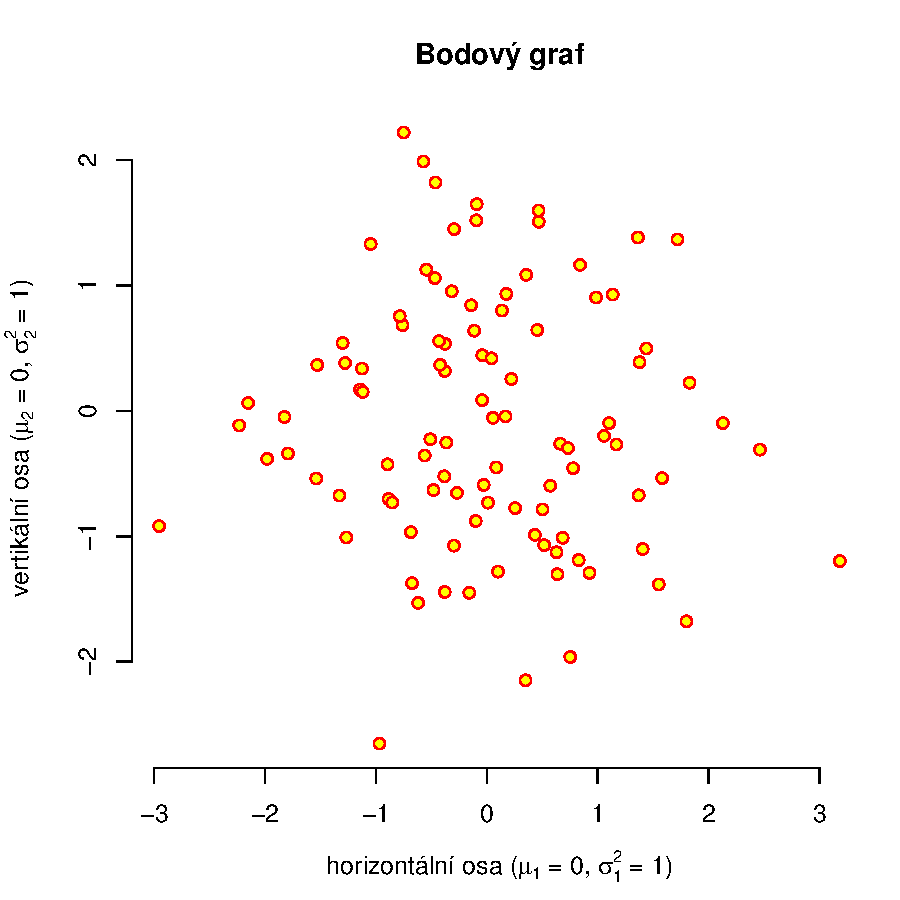
\includegraphics[width=140mm, height=140mm]{img/ukazka-obr01}
% Příponu není potřeba explicitně uvádět, pdflatex automaticky hledá pdf.
% Rozměry také není nutné uvádět.
\caption{Náhodný výběr z~rozdělení $\mathcal{N}_2(\boldsymbol{0},\,I)$.}
\label{obr03:Nvyber}
\end{figure}

\begin{figure}[p]\centering
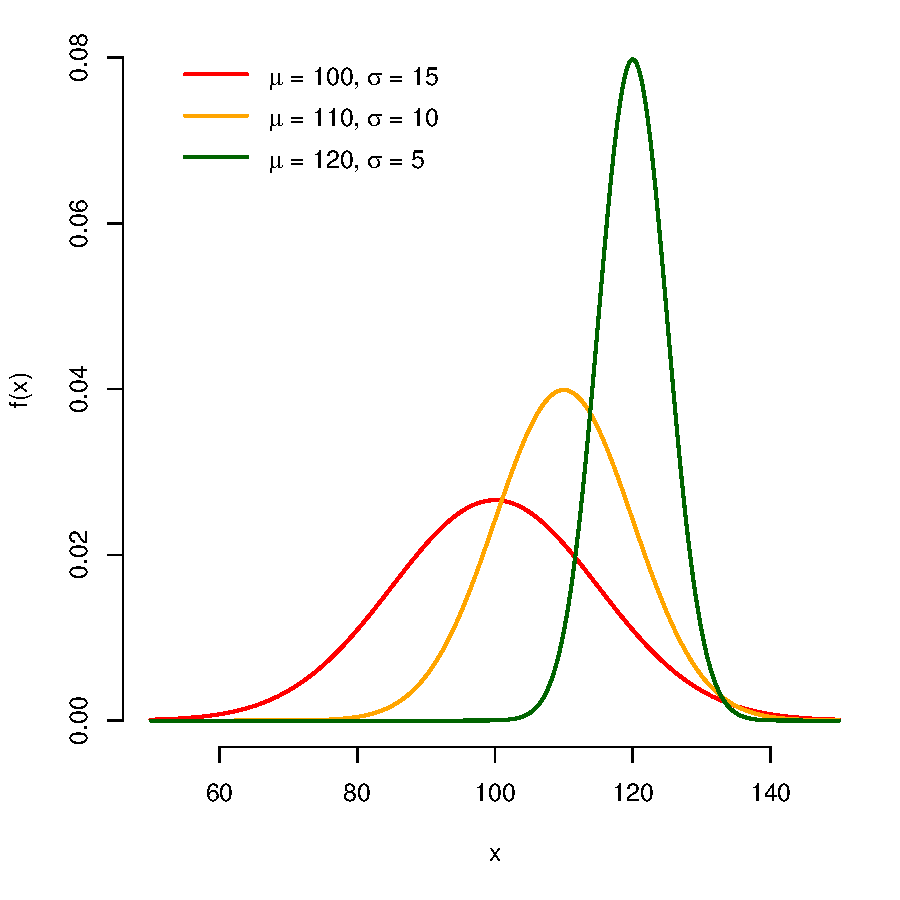
\includegraphics[width=140mm, height=140mm]{img/ukazka-obr02}
\caption{Hustoty několika normálních rozdělení.}
\label{obr03:Nhust}
\end{figure}

\begin{figure}[p]\centering
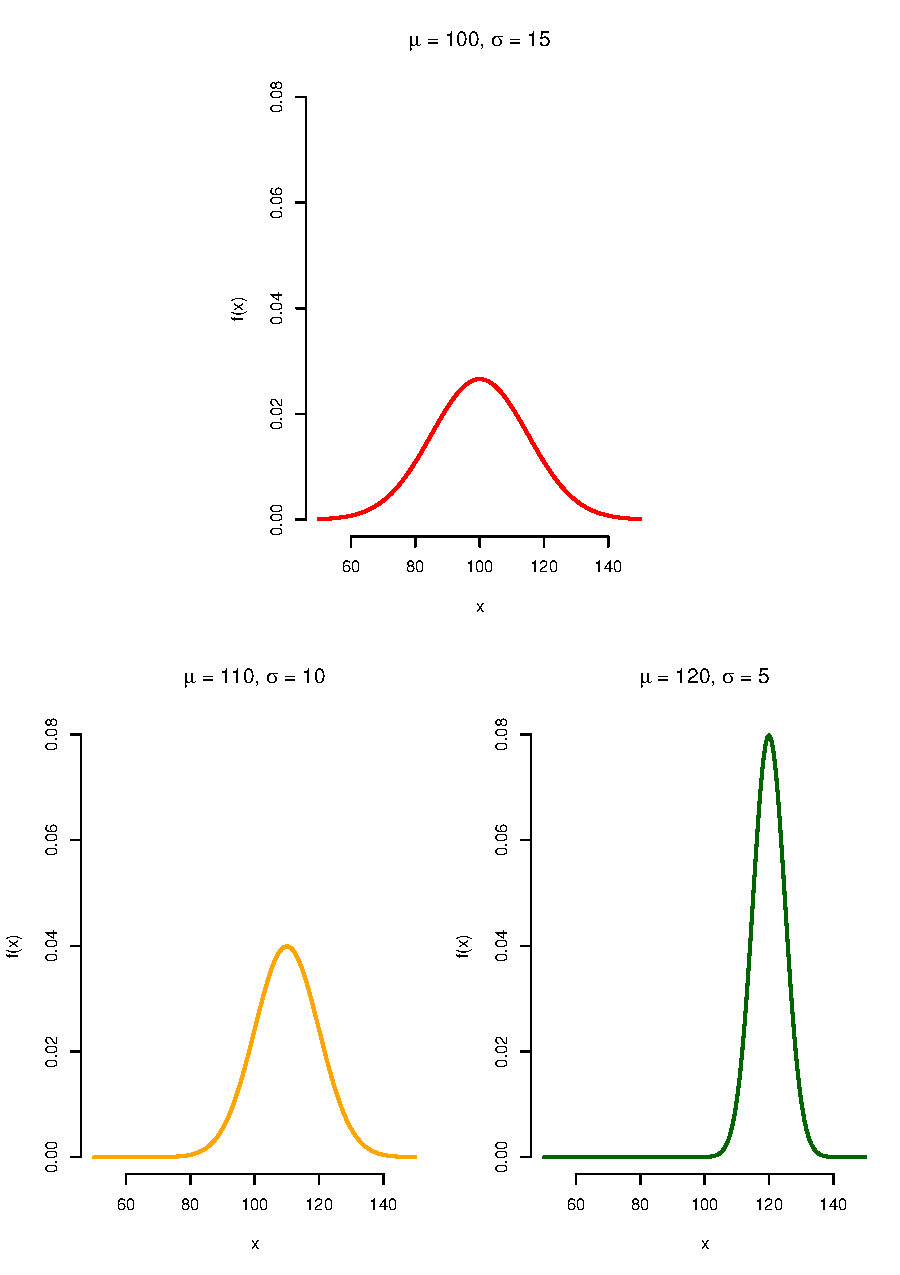
\includegraphics[width=140mm, height=198mm]{img/ukazka-obr03}
\caption{Hustoty několika normálních rozdělení.}
\label{obr03:Nhust:podruhe}

\end{figure}

% %%% Fiktivní kapitola s instrukcemi k PDF/A

\chapter{Formát PDF/A}

Opatření rektora č. 13/2017 určuje, že elektronická podoba závěrečných
prací musí být odevzdávána ve formátu PDF/A úrovně 1a nebo 2u. To jsou
profily formátu PDF určující, jaké vlastnosti PDF je povoleno používat,
aby byly dokumenty vhodné k~dlouhodobé archivaci a dalšímu automatickému
zpracování. Dále se budeme zabývat úrovní 2u, kterou sázíme \TeX{}em.

Mezi nejdůležitější požadavky PDF/A-2u patří:

\begin{itemize}

\item Všechny fonty musí být zabudovány uvnitř dokumentu. Nejsou přípustné
odkazy na externí fonty (ani na \uv{systémové}, jako je Helvetica nebo Times).

\item Fonty musí obsahovat tabulku ToUnicode, která definuje převod z~kódování
znaků použitého uvnitř fontu to Unicode. Díky tomu je možné z~dokumentu
spolehlivě extrahovat text.

\item Dokument musí obsahovat metadata ve formátu XMP a je-li barevný,
pak také formální specifikaci barevného prostoru.

\end{itemize}

Tato šablona používá balíček {\tt pdfx,} který umí \LaTeX{} nastavit tak,
aby požadavky PDF/A splňoval. Metadata v~XMP se generují automaticky podle
informací v~souboru {\tt prace.xmpdata} (na vygenerovaný soubor se můžete
podívat v~{\tt pdfa.xmpi}).

Validitu PDF/A můžete zkontrolovat pomocí nástroje VeraPDF, který je
k~dispozici na \url{http://verapdf.org/}.

Pokud soubor nebude validní, mezi obvyklé příčiny patří používání méně
obvyklých fontů (které se vkládají pouze v~bitmapové podobě a/nebo bez
unicodových tabulek) a vkládání obrázků v~PDF, které samy o~sobě standard
PDF/A nesplňují.

Další postřehy o~práci s~PDF/A najdete na \url{http://mj.ucw.cz/vyuka/bc/pdfaq.html}.


\chapter*{Závěr}
\addcontentsline{toc}{chapter}{Závěr}


%%% Seznam použité literatury
%%% Seznam použité literatury (bibliografie)
%%%
%%% Pro vytváření bibliografie používáme biblatex. Ten zpracovává
%%% citace v textu (např. makro \cite{...}) a vyhledává k nim literaturu
%%% v souboru literatura.bib.
%%%
%%% Podívejte se na nastavení biblatexu v souboru thesis.tex.

%%% Vytvoření seznamu literatury. Pozor, pokud jste necitovali ani jednu
%%% položku, seznam se automaticky vynechá.

% Dovolíme položkám trochu vyčuhovat přes pravý okraj.
\def\bibfont{\hfuzz=2pt}

\printbibliography[heading=bibintoc,title=Literatura]

%%% Kdybyste chtěli bibliografii vytvářet ručně (bez biblatexu), lze to udělat
%%% následovně. V takovém případě se řiďte normou ISO 690 a zvyklostmi v oboru.

% \begin{thebibliography}{99}
%
% \bibitem{lamport94}
%   {\sc Lamport,} Leslie.
%   \emph{\LaTeX: A Document Preparation System}.
%   2. vydání.
%   Massachusetts: Addison Wesley, 1994.
%   ISBN 0-201-52983-1.
%
% \end{thebibliography}


%%% Obrázky v práci
%%% (pokud jich je malé množství, obvykle není třeba seznam uvádět)
\listoffigures

%%% Tabulky v práci (opět nemusí být nutné uvádět)
%%% U matematických prací může být lepší přemístit seznam tabulek na začátek práce.
% \listoftables

%%% Použité zkratky v práci (opět nemusí být nutné uvádět)
%%% U matematických prací může být lepší přemístit seznam zkratek na začátek práce.
\chapwithtoc{Seznam použitých zkratek}
\begin{itemize}
    \item OB - orientačný beh
    \item GUI - grafické užívateľské rozhranie (graphical user interface)
    \item XAML - Extension application markup language
    \item MVVM - Model-View-ViewModel
\end{itemize}



%%% Součástí doktorských prací musí být seznam vlastních publikací
\ifx\ThesisType\TypePhD
\chapwithtoc{Seznam publikací}
\fi

%%% Přílohy k práci, existují-li. Každá příloha musí být alespoň jednou
%%% odkazována z vlastního textu práce. Přílohy se číslují.
%%%
%%% Do tištěné verze se spíše hodí přílohy, které lze číst a prohlížet (dodatečné
%%% tabulky a grafy, různé textové doplňky, ukázky výstupů z počítačových programů,
%%% apod.). Do elektronické verze se hodí přílohy, které budou spíše používány
%%% v elektronické podobě než čteny (zdrojové kódy programů, datové soubory,
%%% interaktivní grafy apod.). Elektronické přílohy se nahrávají do SISu.
%%% Povolené formáty souborů specifikuje opatření rektora č. 72/2017.
%%% Výjimky schvaluje fakultní koordinátor pro zavěrečné práce.
\appendix
\chapter{Přílohy}

\section{První příloha}

\end{document}
